\chapter{Hyperparameters}
\section{K-Means}
For selecting the appropriate amount of clusters, we used an "elbow" plot in combination with the silhouette score.
\begin{enumerate}
  \item Seeds dataset: 4 clusters (see figure: \ref{hyperparameters:k-means-seeds-dataset})
  \item Heart dataset: TODO
  \item Circle dataset: 5 clusters (see figure: \ref{hyperparameters:k-means-circle-dataset})
  \item Line dataset: 4 clusters (see figure: \ref{hyperparameters:k-means-line-dataset})
  \item Skewed dataset: 4 clusters (see figure: \ref{hyperparameters:k-means-skewed-dataset})
\end{enumerate}
\begin{figure}[H]
  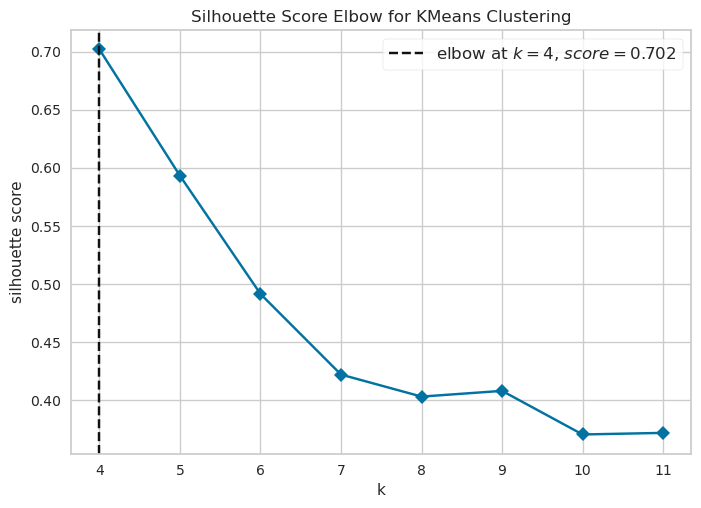
\includegraphics[width=0.6\textwidth]{Appendix/parameter-selection/selecting-k.png}
  \caption{Selecting the $k$ for K-Means for seeds dataset using the "elbow plot" using section \ref{theory:kmeans}}
  \label{hyperparameters:k-means-seeds-dataset}
\end{figure}

\begin{figure}[H]
  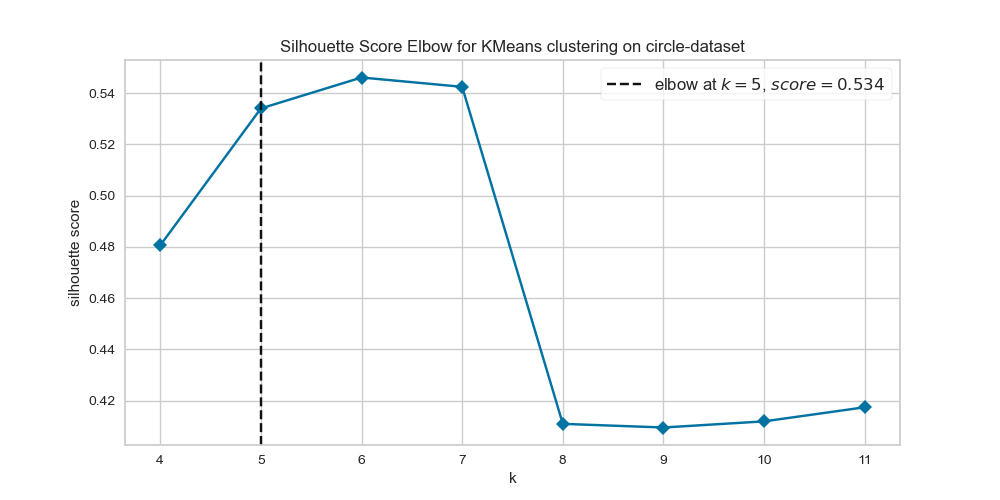
\includegraphics[width=0.6\textwidth]{Method/images/synthetic-datasets-k/circle-dataset_elbow.png}
  \caption{Selecting the $k$ for K-Means for the circle dataset using the "elbow plot" using section \ref{theory:kmeans}}
  \label{hyperparameters:k-means-circle-dataset}
\end{figure}


\begin{figure}[H]
  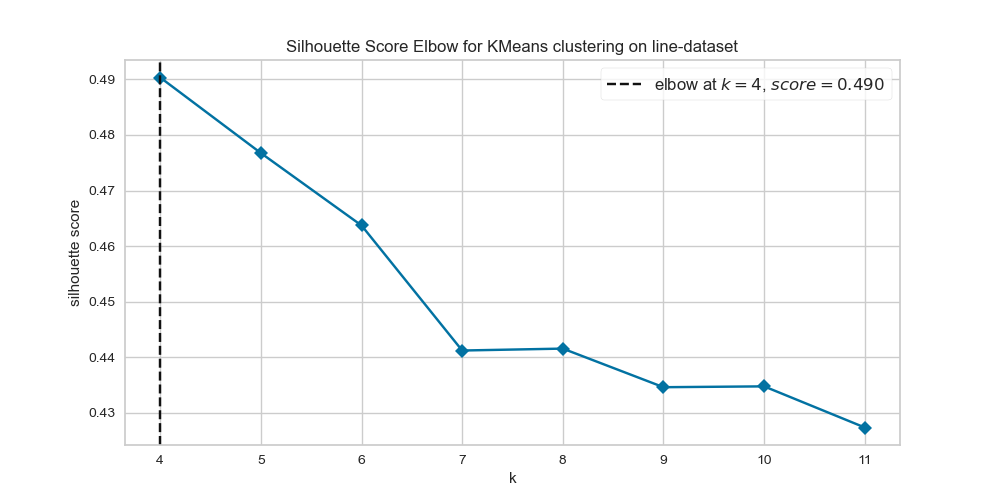
\includegraphics[width=0.6\textwidth]{Method/images/synthetic-datasets-k/line-dataset_elbow.png}
  \caption{Selecting the $k$ for K-Means for the line dataset using the "elbow plot" using section \ref{theory:kmeans}}
  \label{hyperparameters:k-means-line-dataset}
\end{figure}

\begin{figure}[H]
  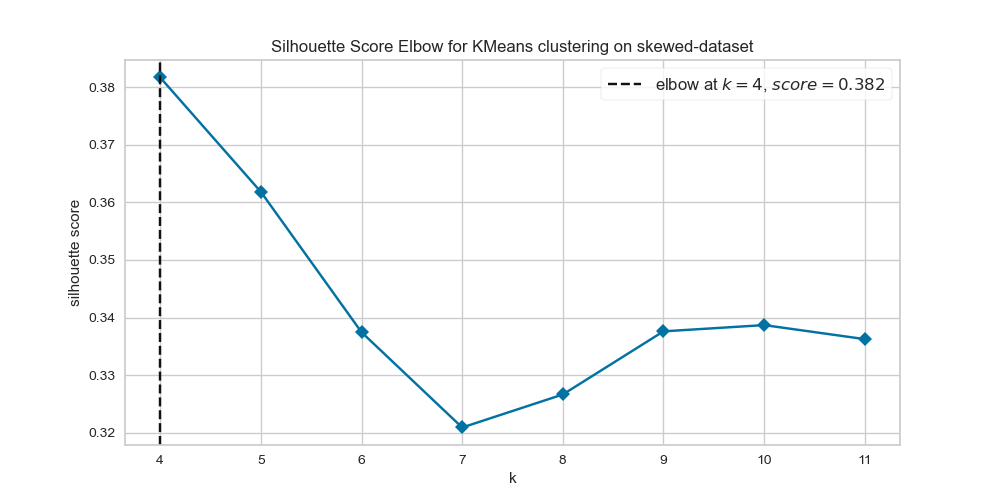
\includegraphics[width=0.6\textwidth]{Method/images/synthetic-datasets-k/skewed-dataset_elbow.png}
  \caption{Selecting the $k$ for K-Means for the skewed dataset using the "elbow plot" using section \ref{theory:kmeans}}
  \label{hyperparameters:k-means-skewed-dataset}
\end{figure}

\section{Agglomerative clustering} \label{appendix:agglomerative-hyperparameters}

\subsection{Seeds dataset}
\begin{figure}[H]
  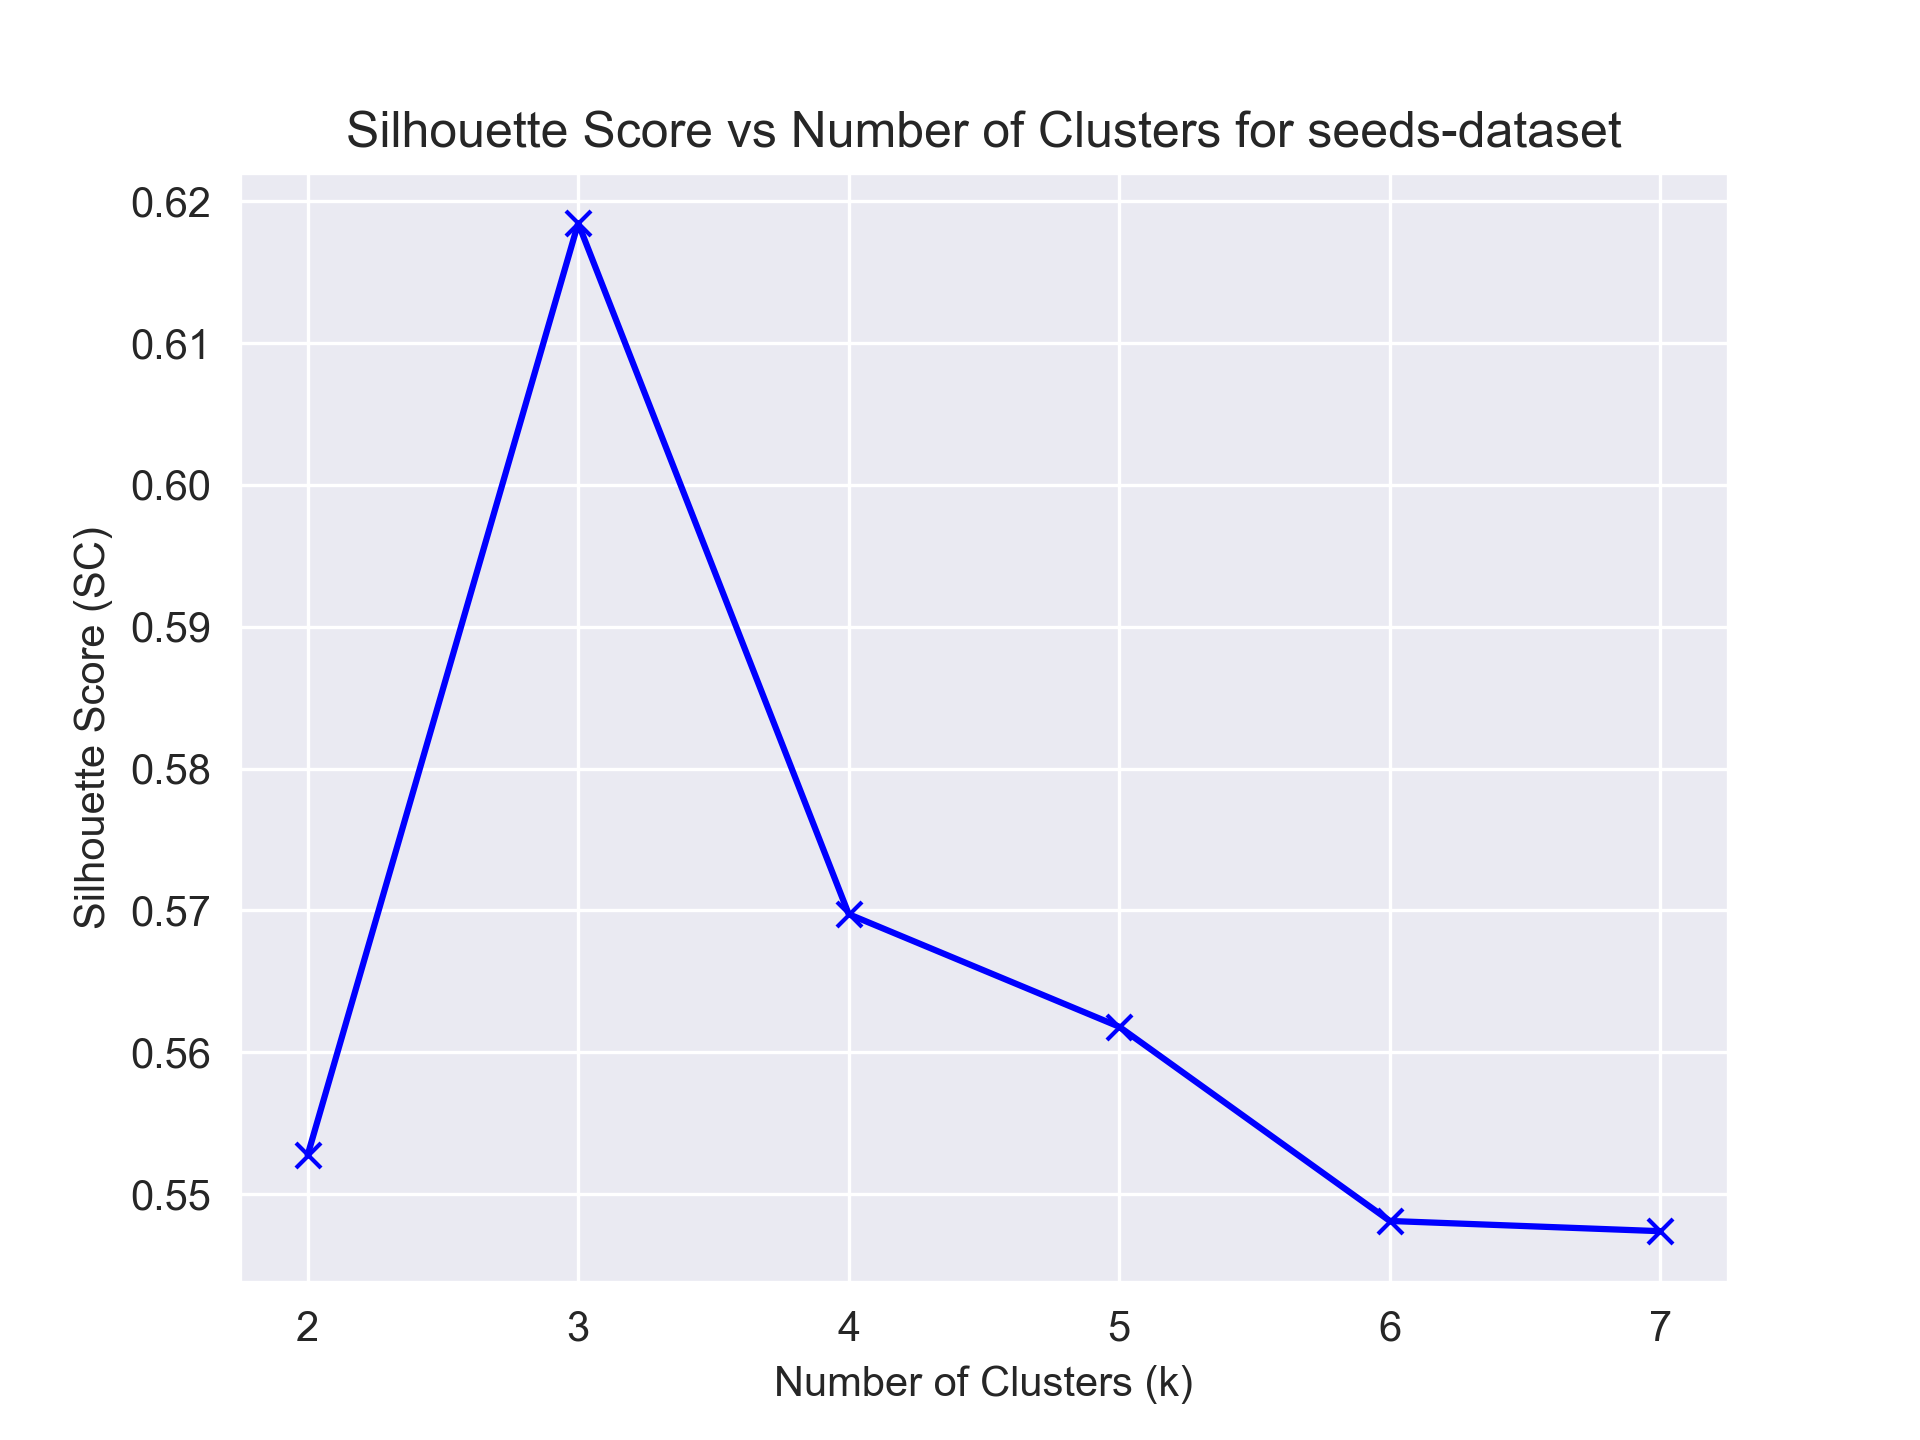
\includegraphics[width=0.8\textwidth]{Appendix/parameter-selection/seeds-dataset_agglomerative_optimal_cluster_2.png}
  \caption{Selecting the $k$ for Agglomerative clustering for seeds dataset (2 dimensions) using the "elbow plot."}
  \label{hyperparameters:agglomerative-seeds-dataset-2d}
\end{figure}
\begin{figure}[H]
  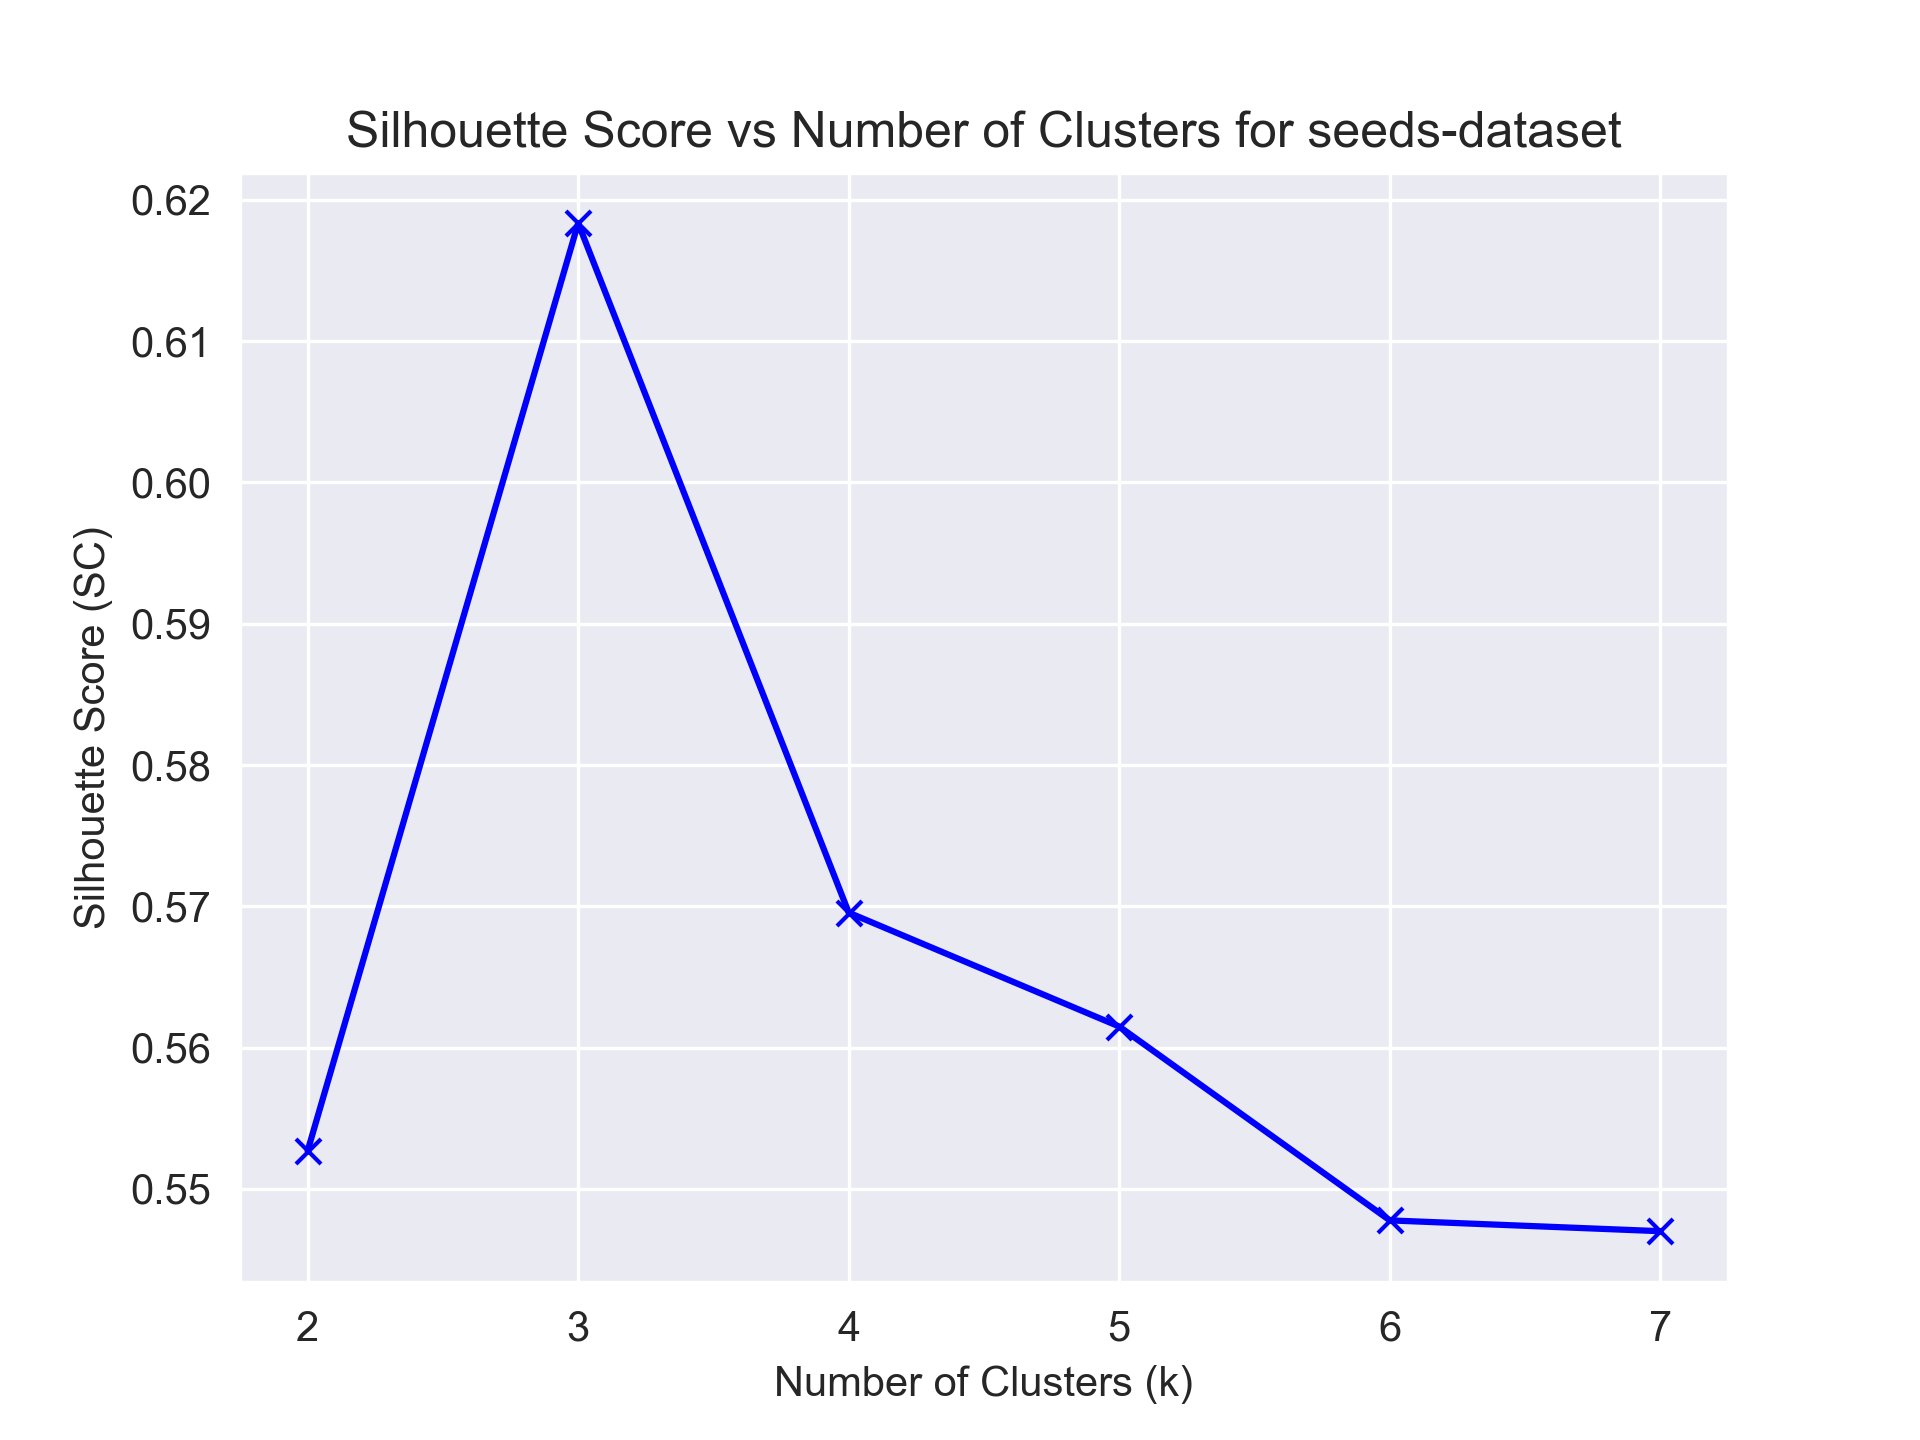
\includegraphics[width=0.8\textwidth]{Appendix/parameter-selection/seeds-dataset_agglomerative_optimal_cluster_3.png}
  \caption{Selecting the $k$ for Agglomerative clustering for seeds dataset (3 dimensions) using the "elbow plot."}
  \label{hyperparameters:agglomerative-seeds-dataset-3d}
\end{figure}
\begin{figure}[H]
  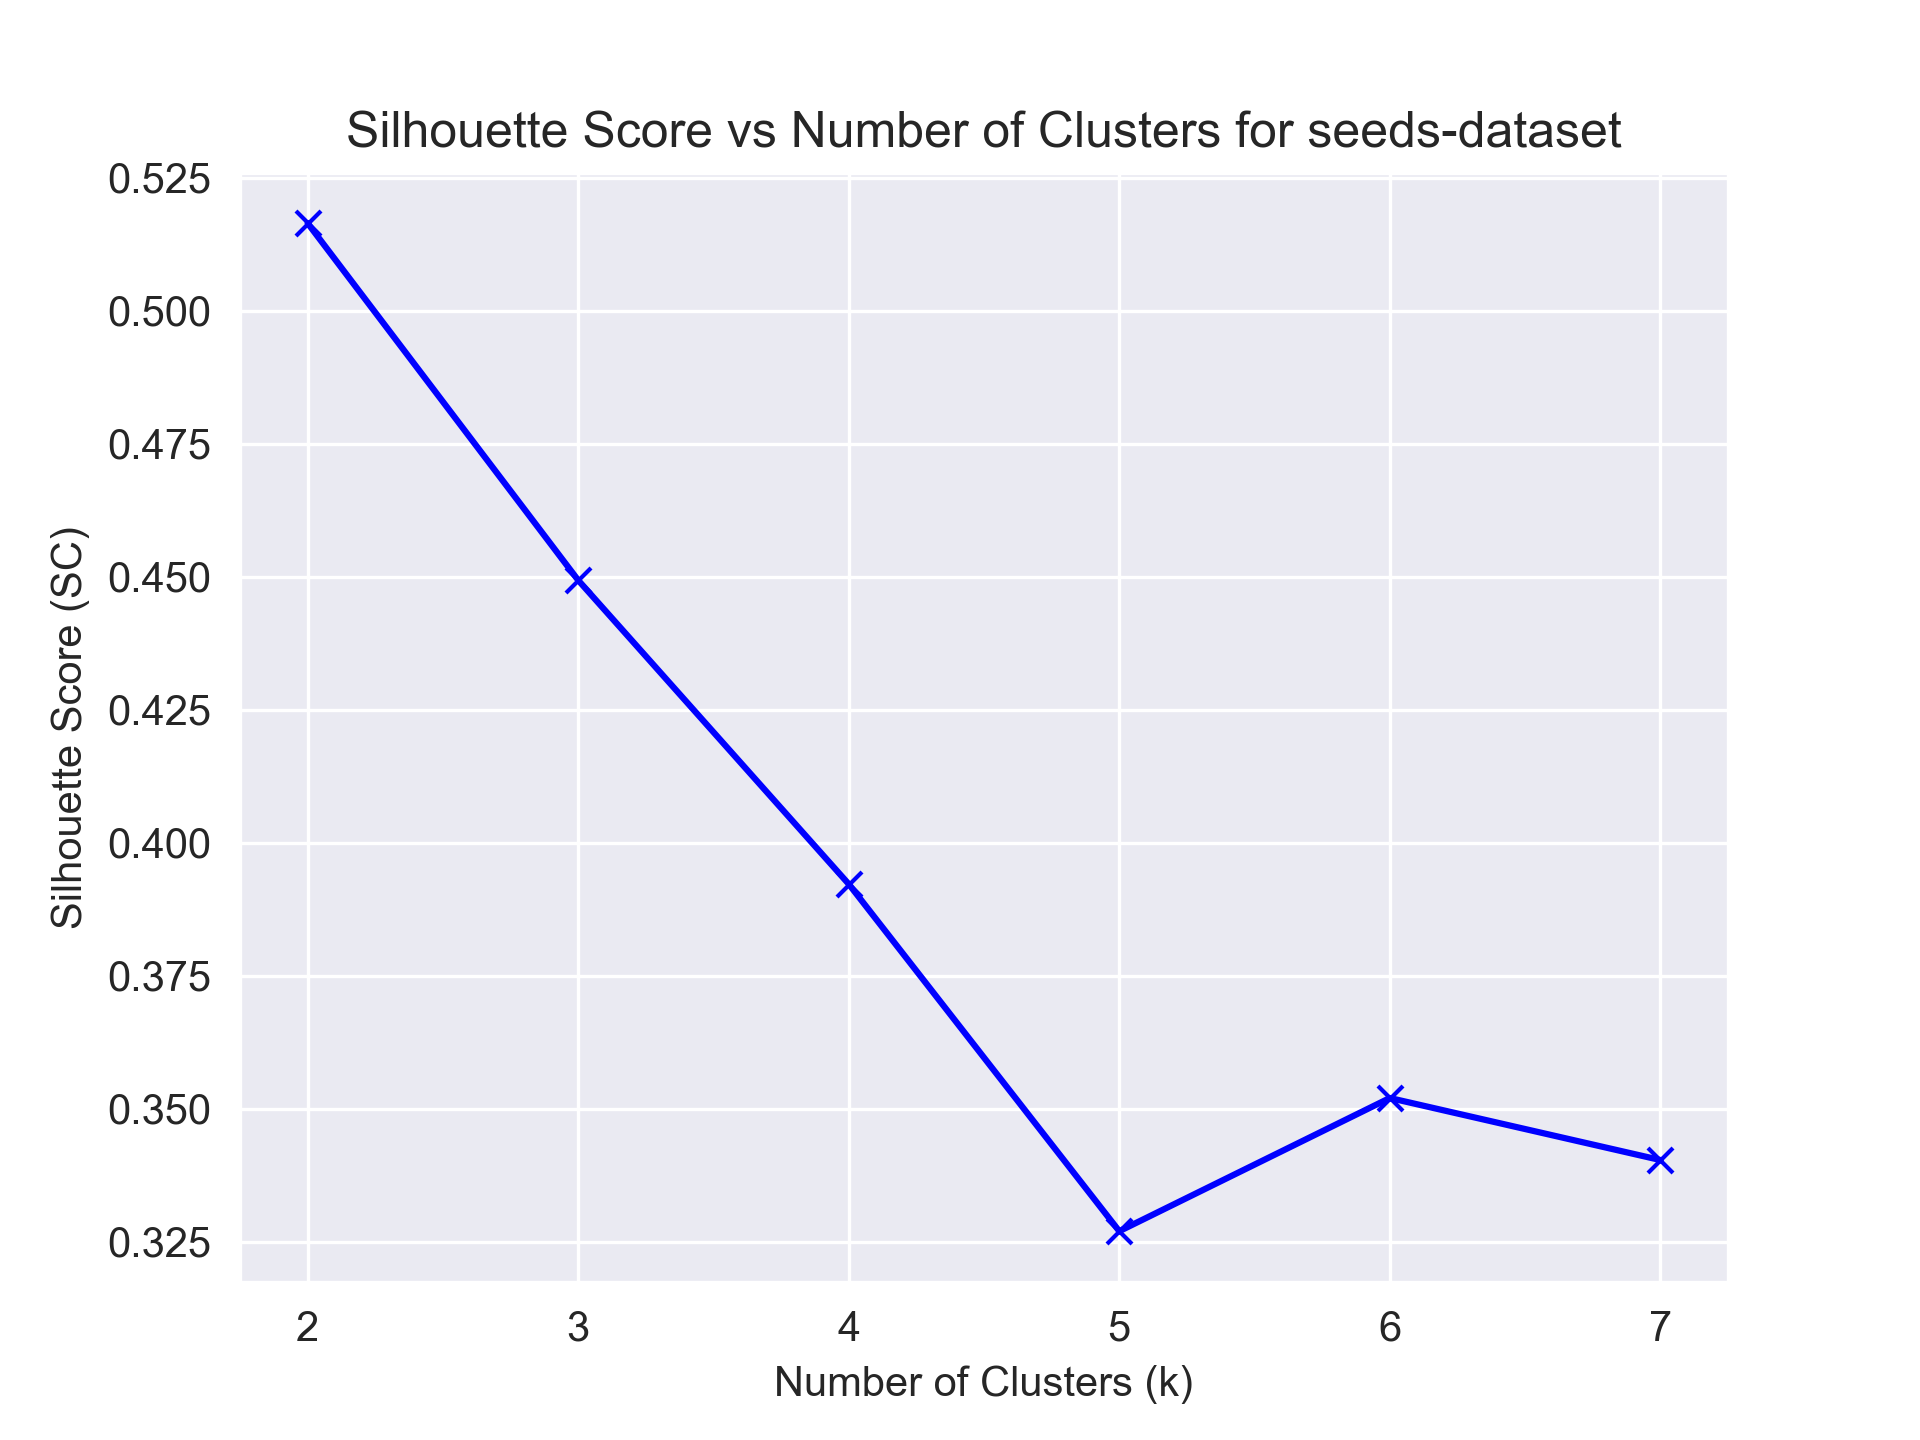
\includegraphics[width=0.8\textwidth]{Appendix/parameter-selection/seeds-dataset_agglomerative_optimal_cluster_7.png}
  \caption{Selecting the $k$ for Agglomerative clustering for seeds dataset (7 dimensions) using the "elbow plot."}
  \label{hyperparameters:agglomerative-seeds-dataset-7d}
\end{figure}
\newpage

\subsection{Heart dataset}
\begin{figure}[H]
  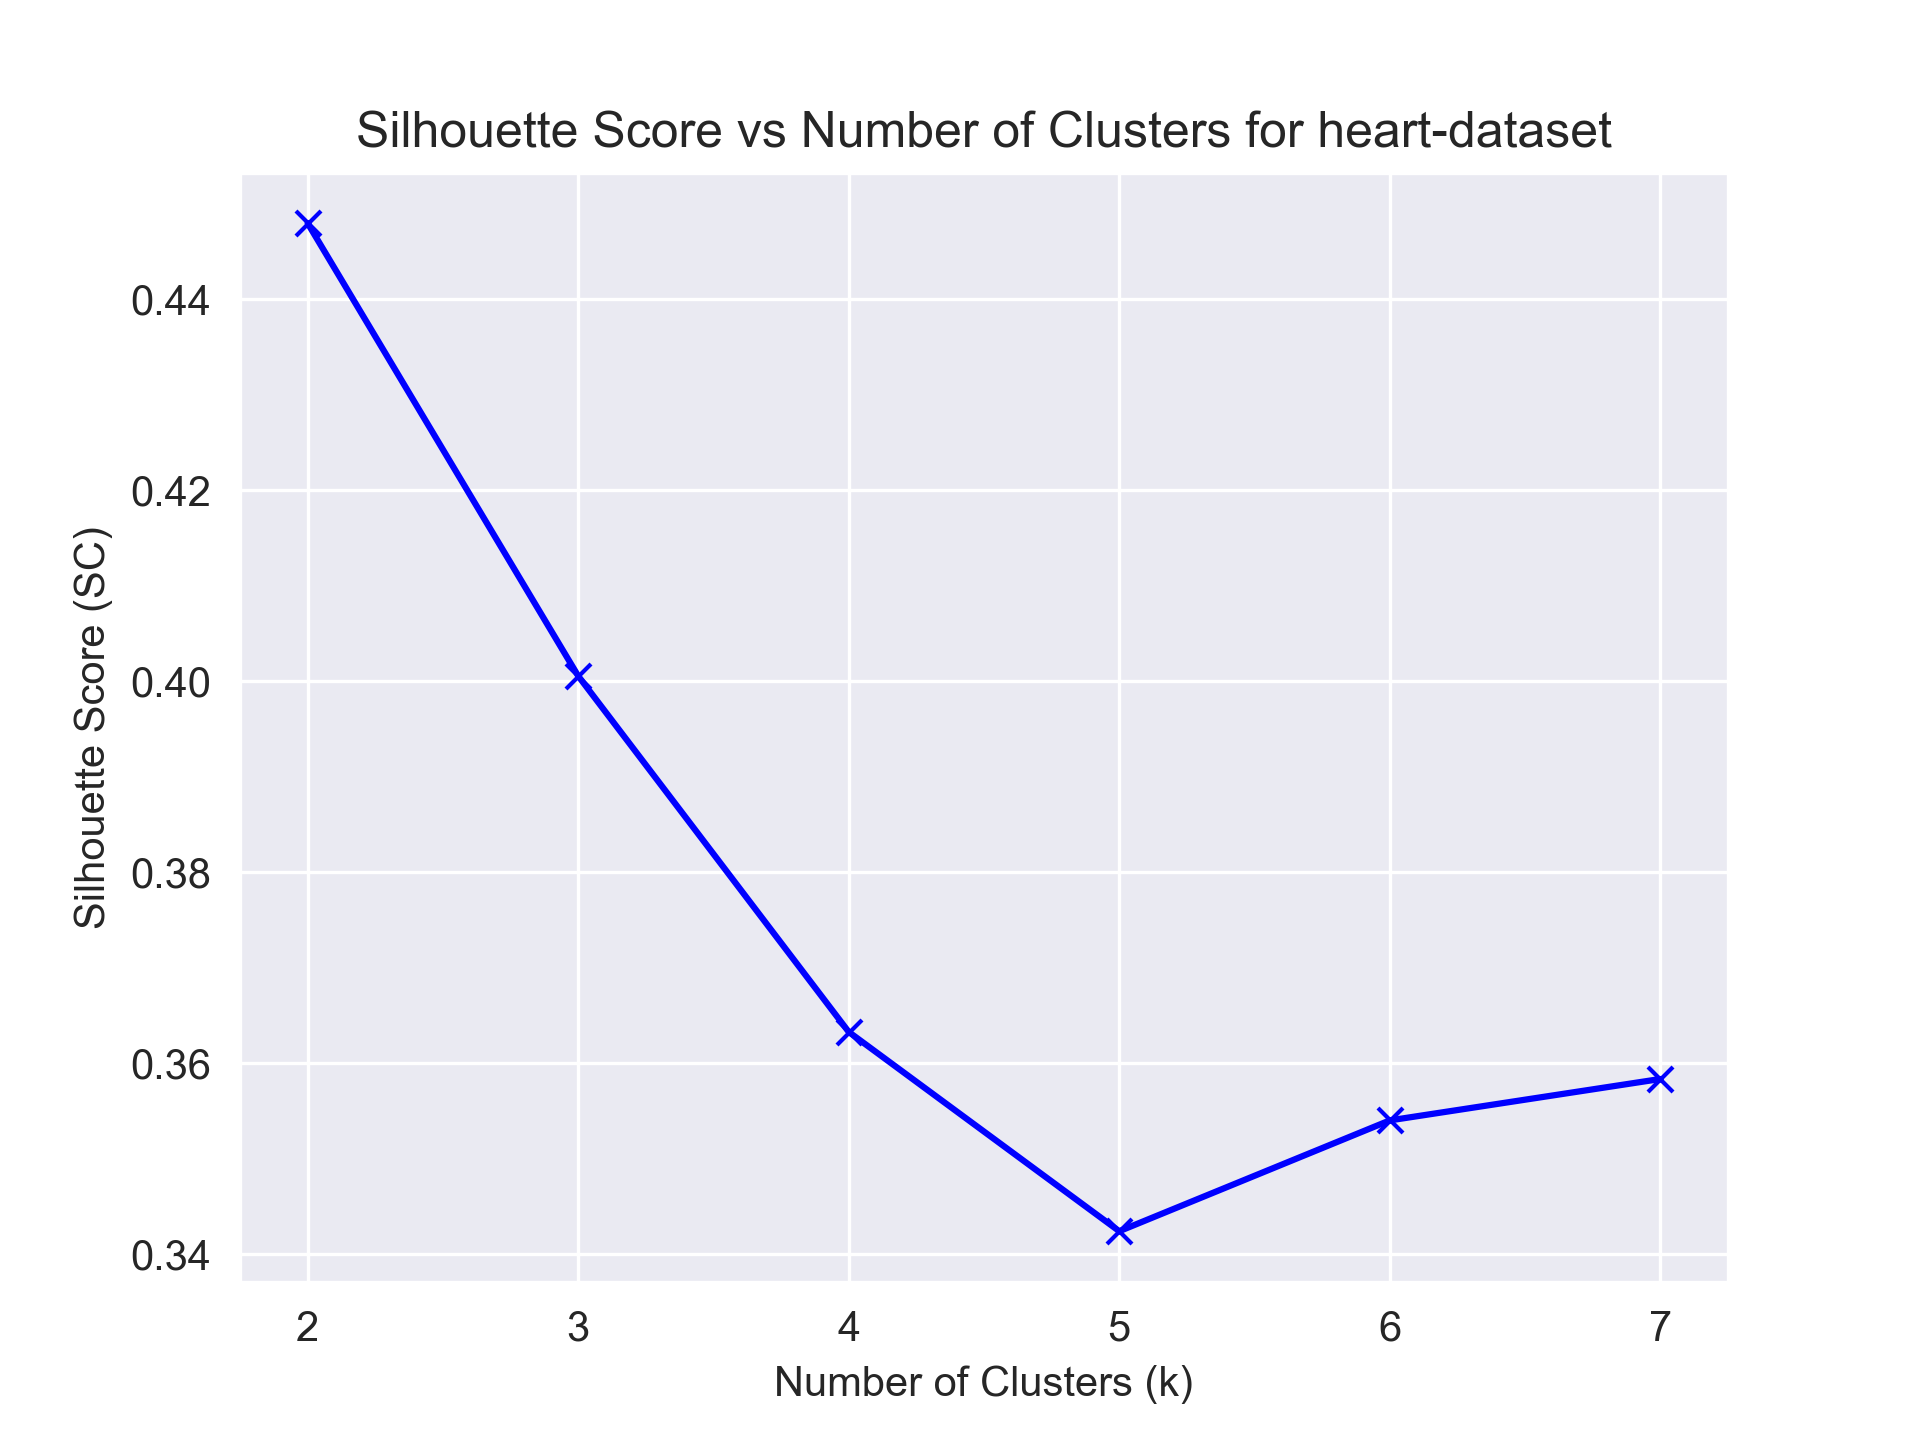
\includegraphics[width=0.8\textwidth]{Appendix/parameter-selection/heart-dataset_agglomerative_optimal_cluster_2.png}
  \caption{Selecting the $k$ for Agglomerative clustering for Heart dataset (2 dimensions) using the "elbow plot."}
  \label{hyperparameters:agglomerative-heart-dataset-2d}
\end{figure}
\begin{figure}[H]
  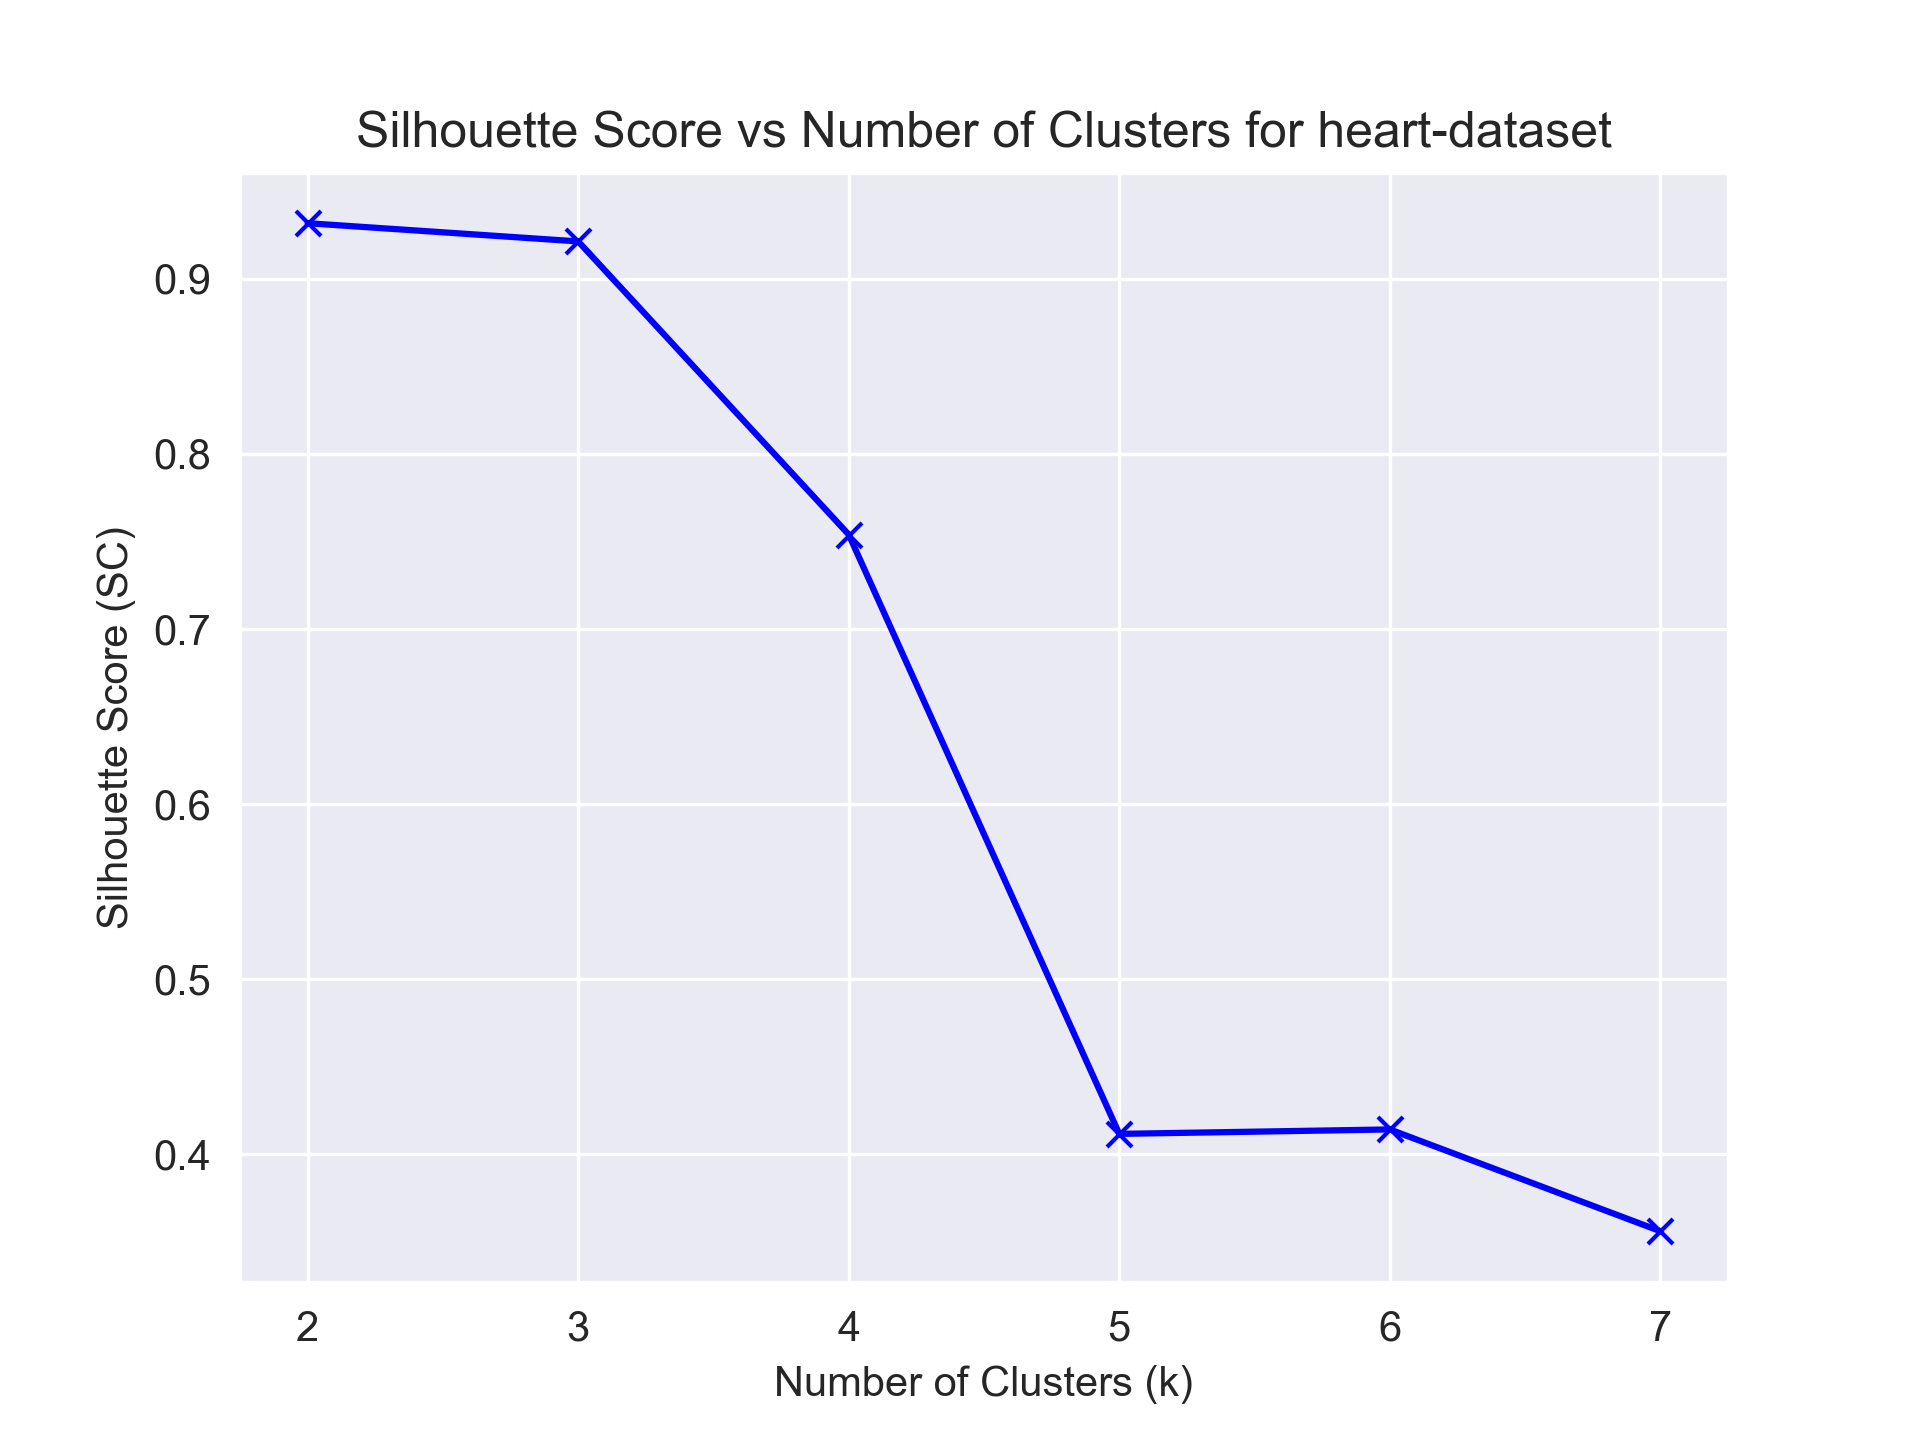
\includegraphics[width=0.8\textwidth]{Appendix/parameter-selection/heart-dataset_agglomerative_optimal_cluster_3.png}
  \caption{Selecting the $k$ for Agglomerative clustering for Heart dataset (3 dimensions) using the "elbow plot."}
  \label{hyperparameters:agglomerative-heart-dataset-3d}
\end{figure}
\begin{figure}[H]
  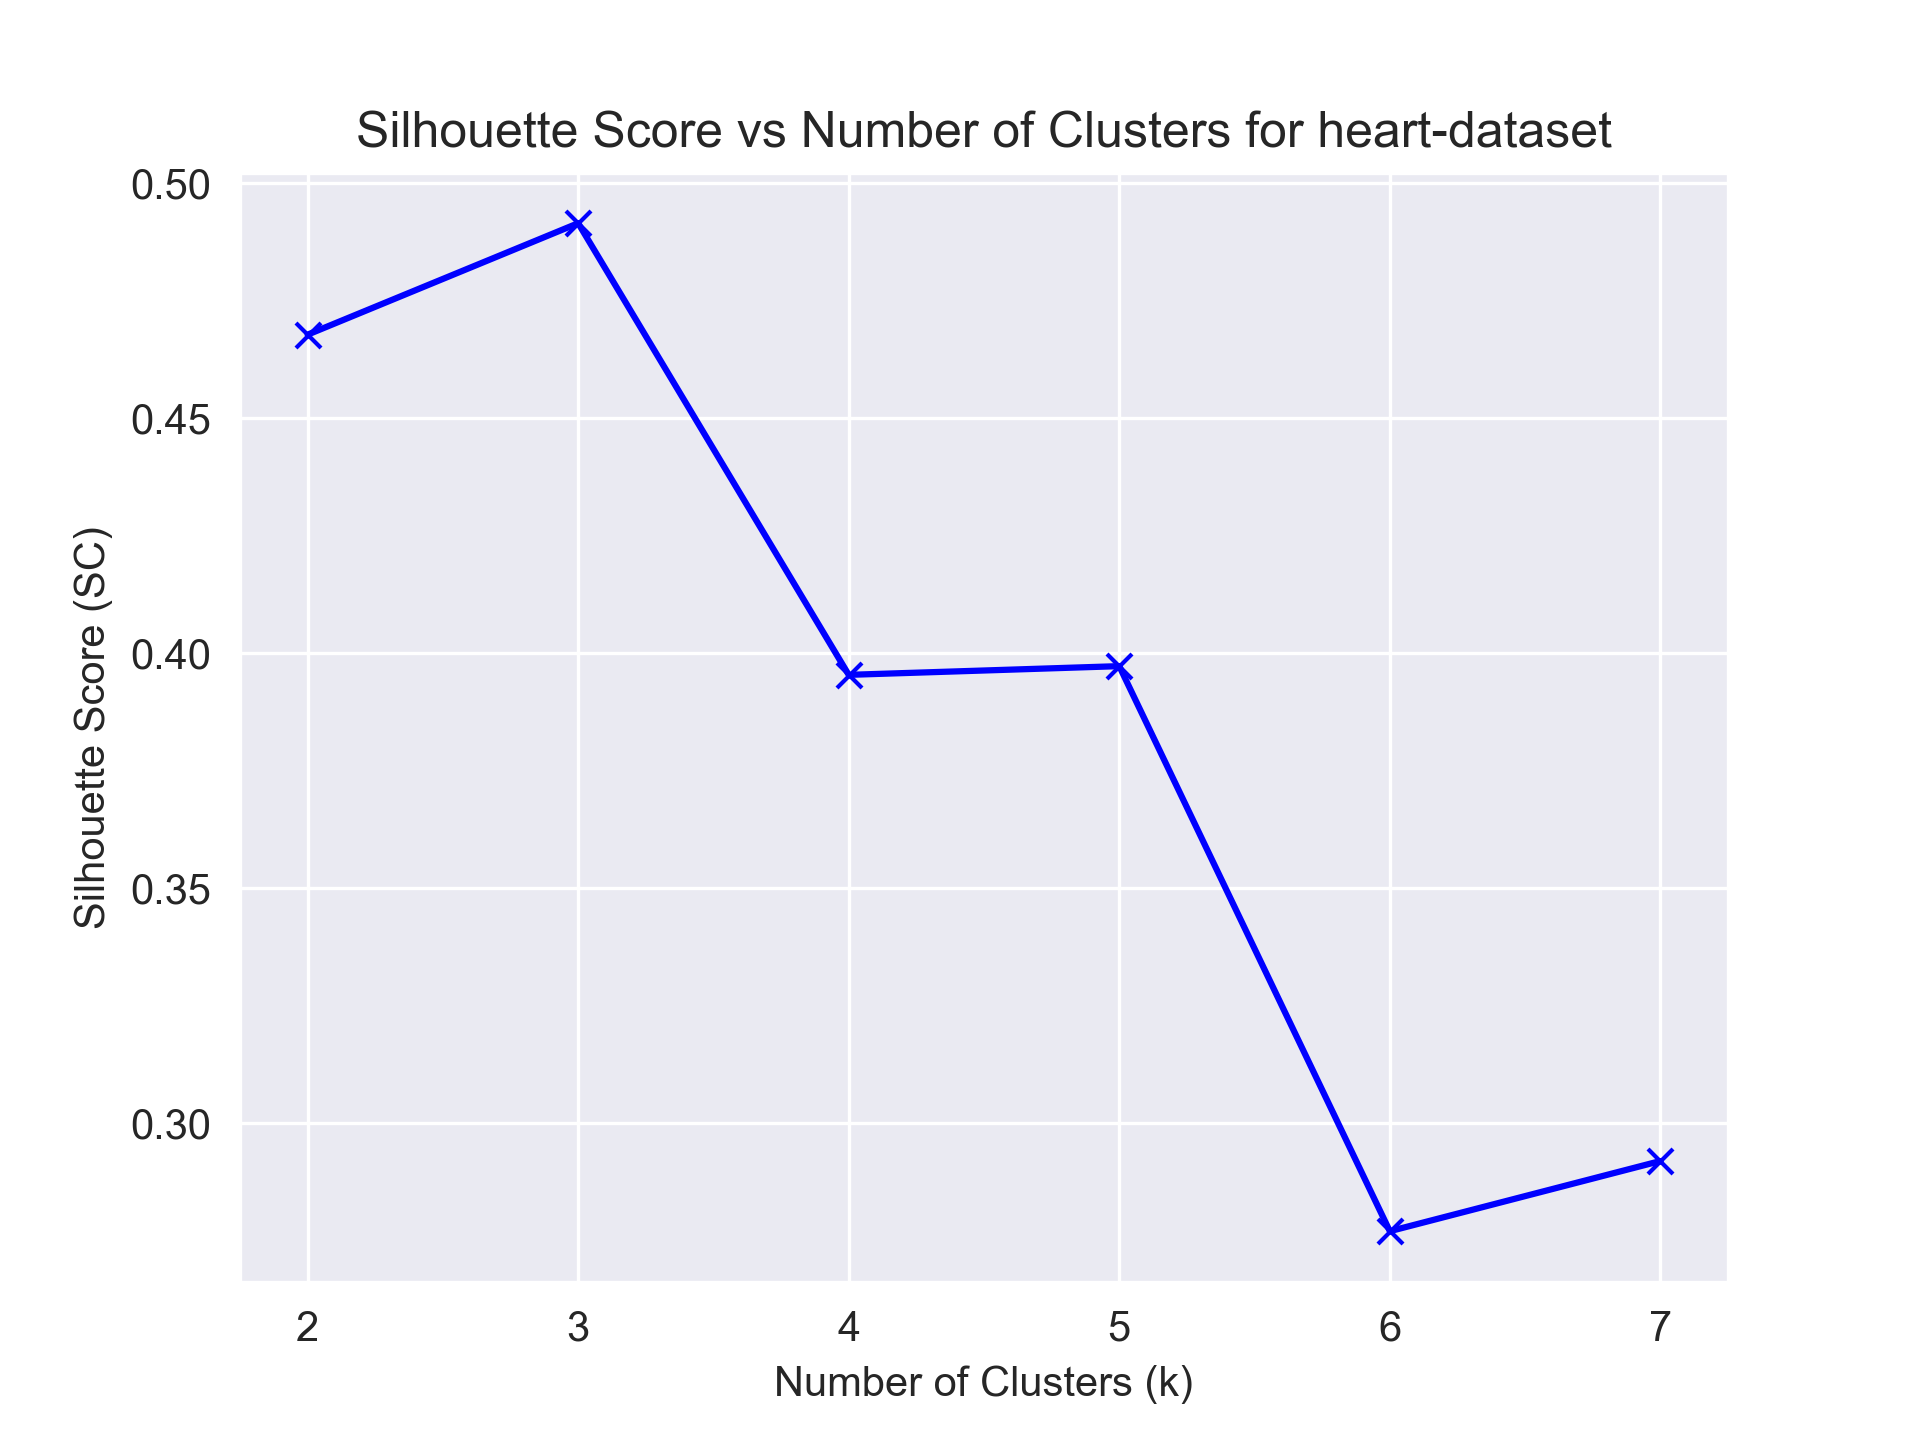
\includegraphics[width=0.8\textwidth]{Appendix/parameter-selection/heart-dataset_agglomerative_optimal_cluster_9.png}
  \caption{Selecting the $k$ for Agglomerative clustering for Heart dataset (9 dimensions) using the "elbow plot."}
  \label{hyperparameters:agglomerative-heart-dataset-9d}
\end{figure}
\newpage

\subsection{Circle dataset}

\begin{figure}[H]
  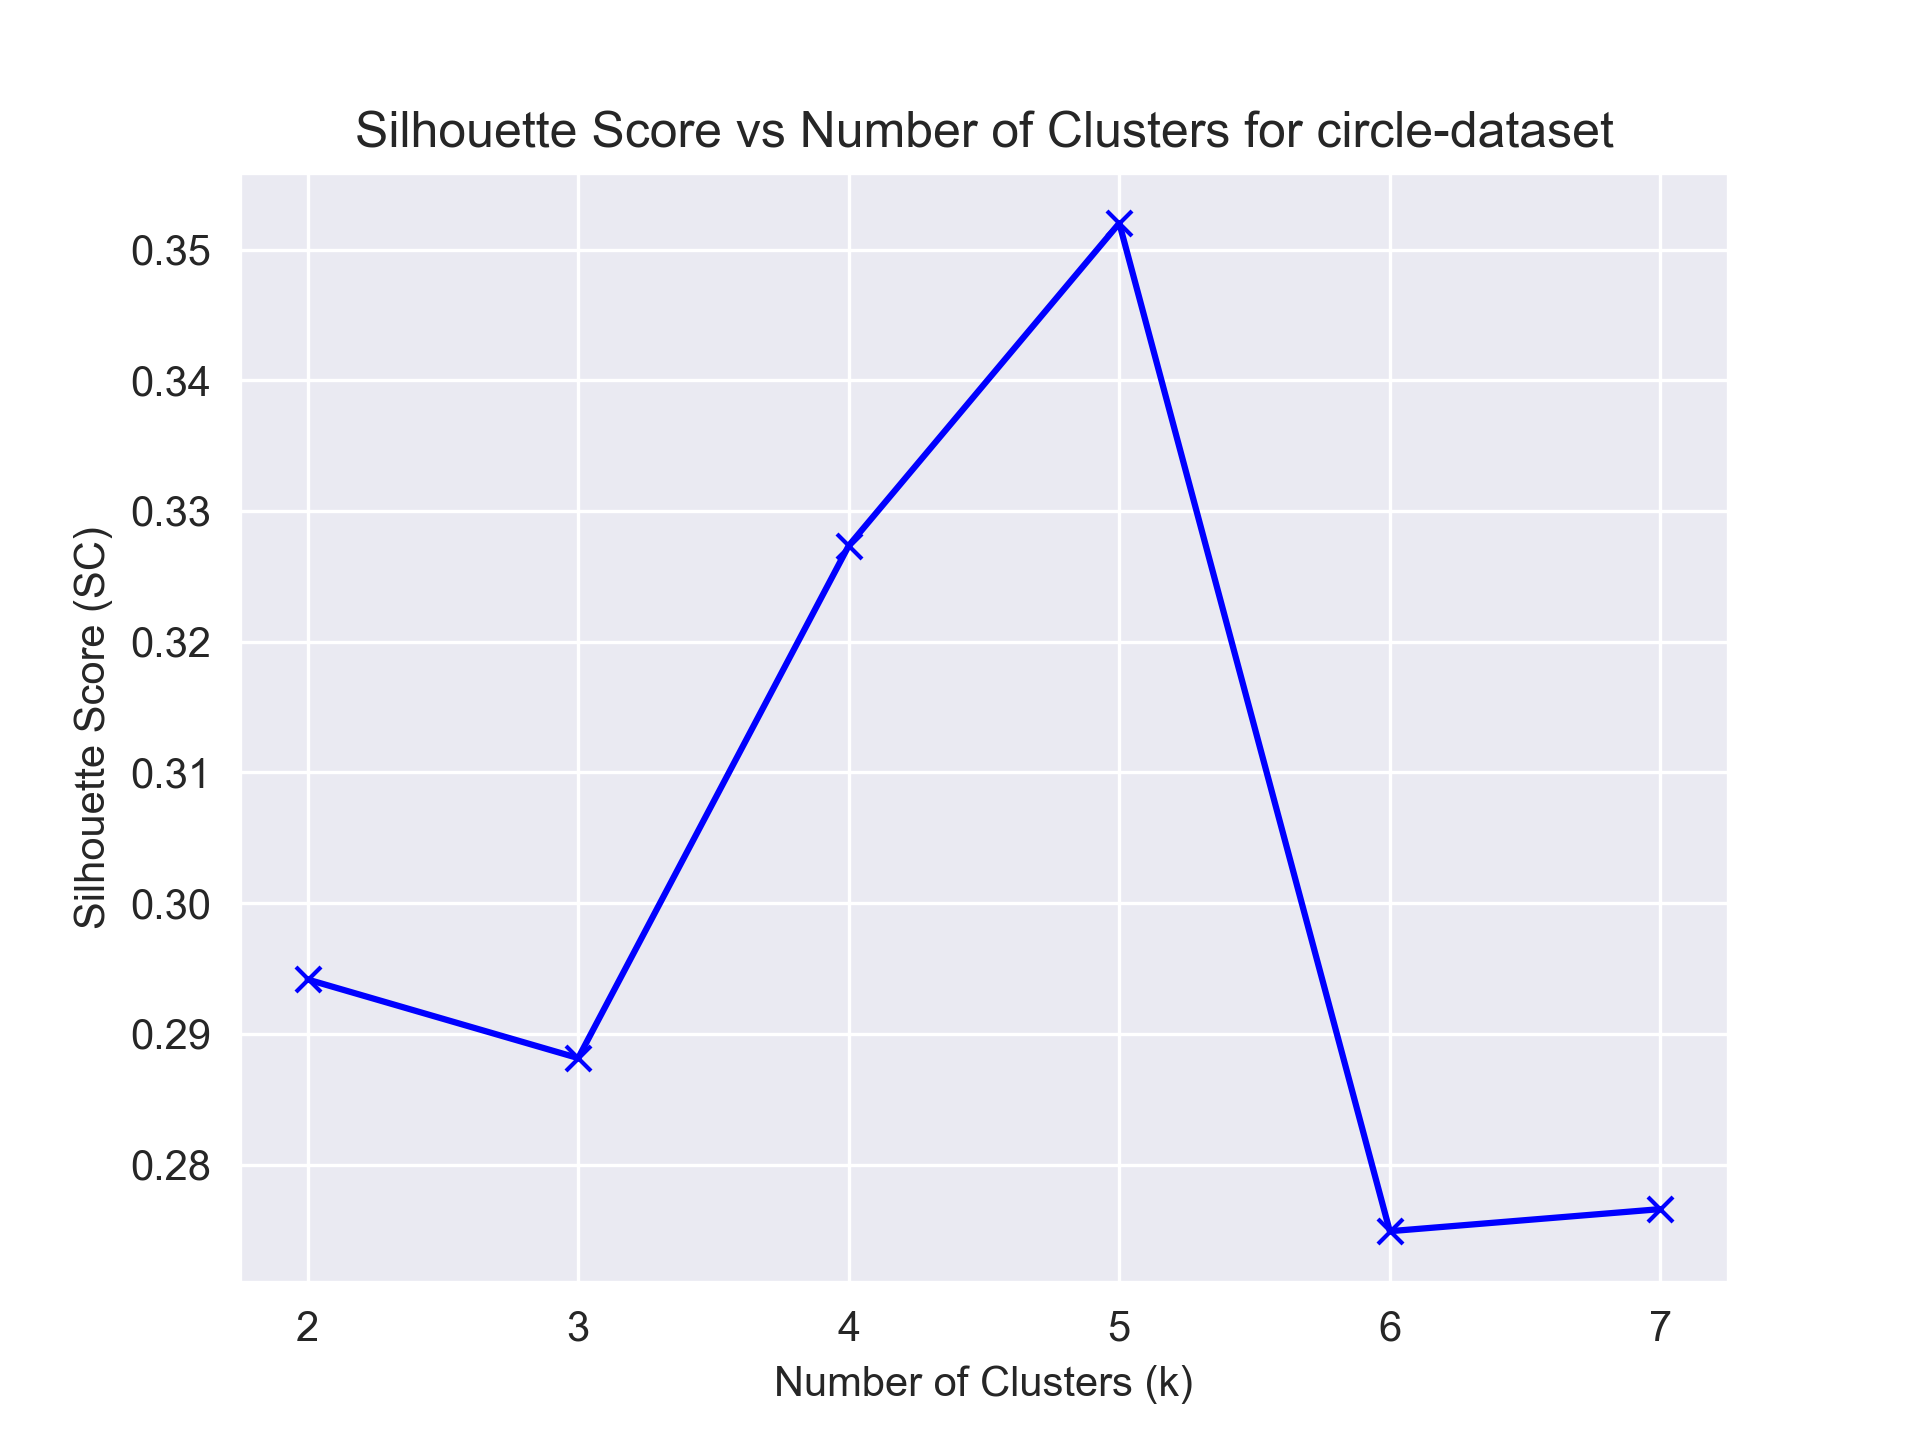
\includegraphics[width=0.8\textwidth]{Appendix/parameter-selection/circle-dataset_agglomerative_optimal_cluster_2.png}
  \caption{Selecting the $k$ for Agglomerative clustering for circle dataset (2-dimensions) using the "elbow plot."}
  \label{hyperparameters:agglomerative-circle-dataset-2d}
\end{figure}
\begin{figure}[H]
  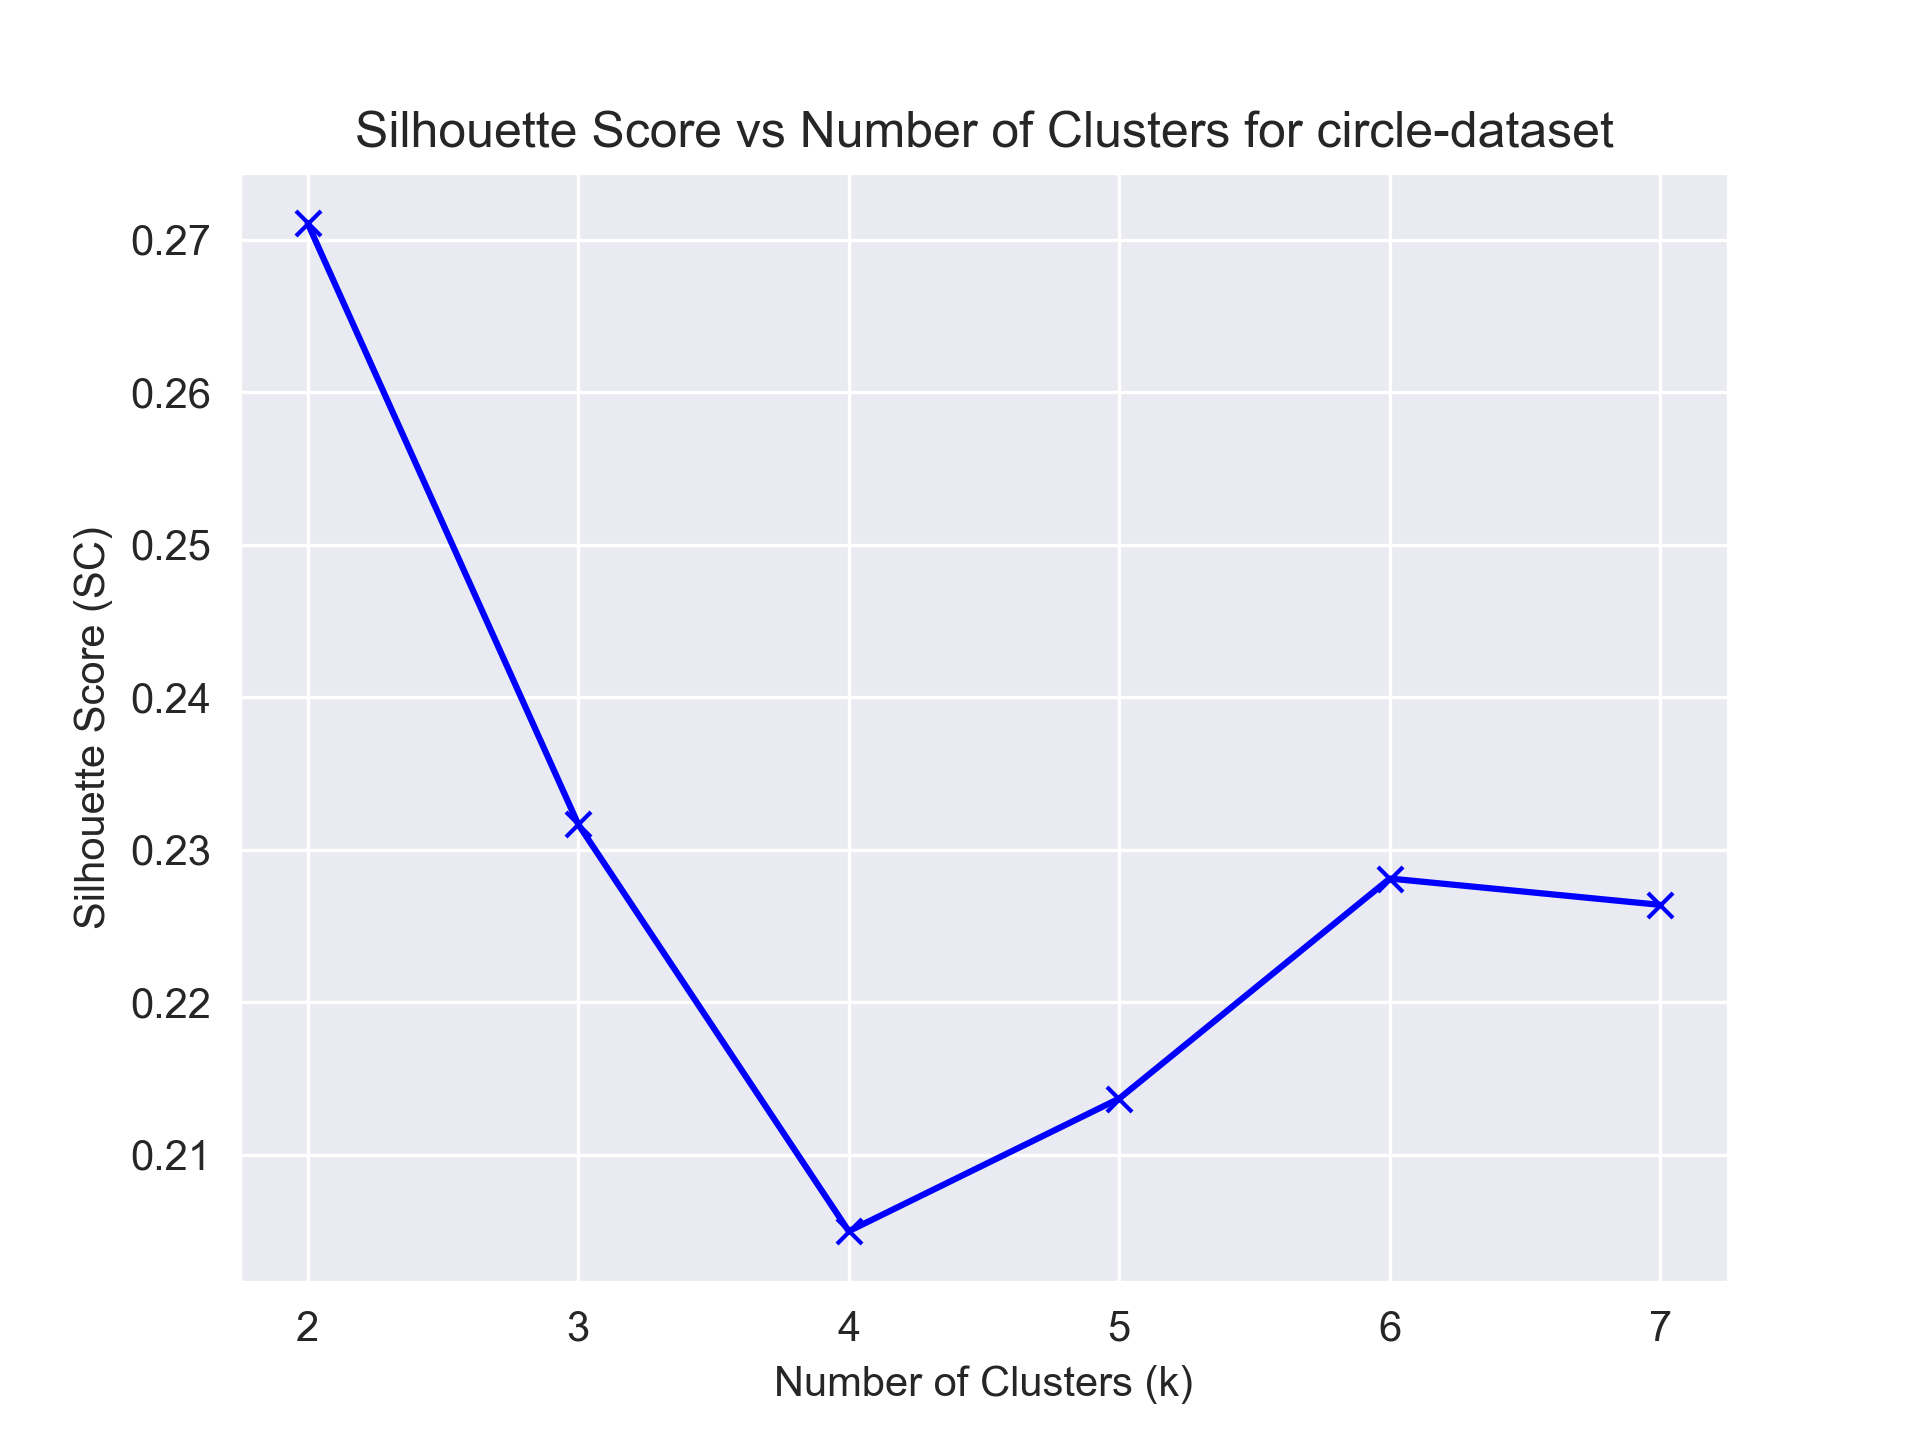
\includegraphics[width=0.8\textwidth]{Appendix/parameter-selection/circle-dataset_agglomerative_optimal_cluster_3.png}
  \caption{Selecting the $k$ for Agglomerative clustering for circle dataset (3-dimensions) using the "elbow plot."}
  \label{hyperparameters:agglomerative-circle-dataset-3d}
\end{figure}
\newpage

\subsection{Line dataset}
\begin{figure}[H]
  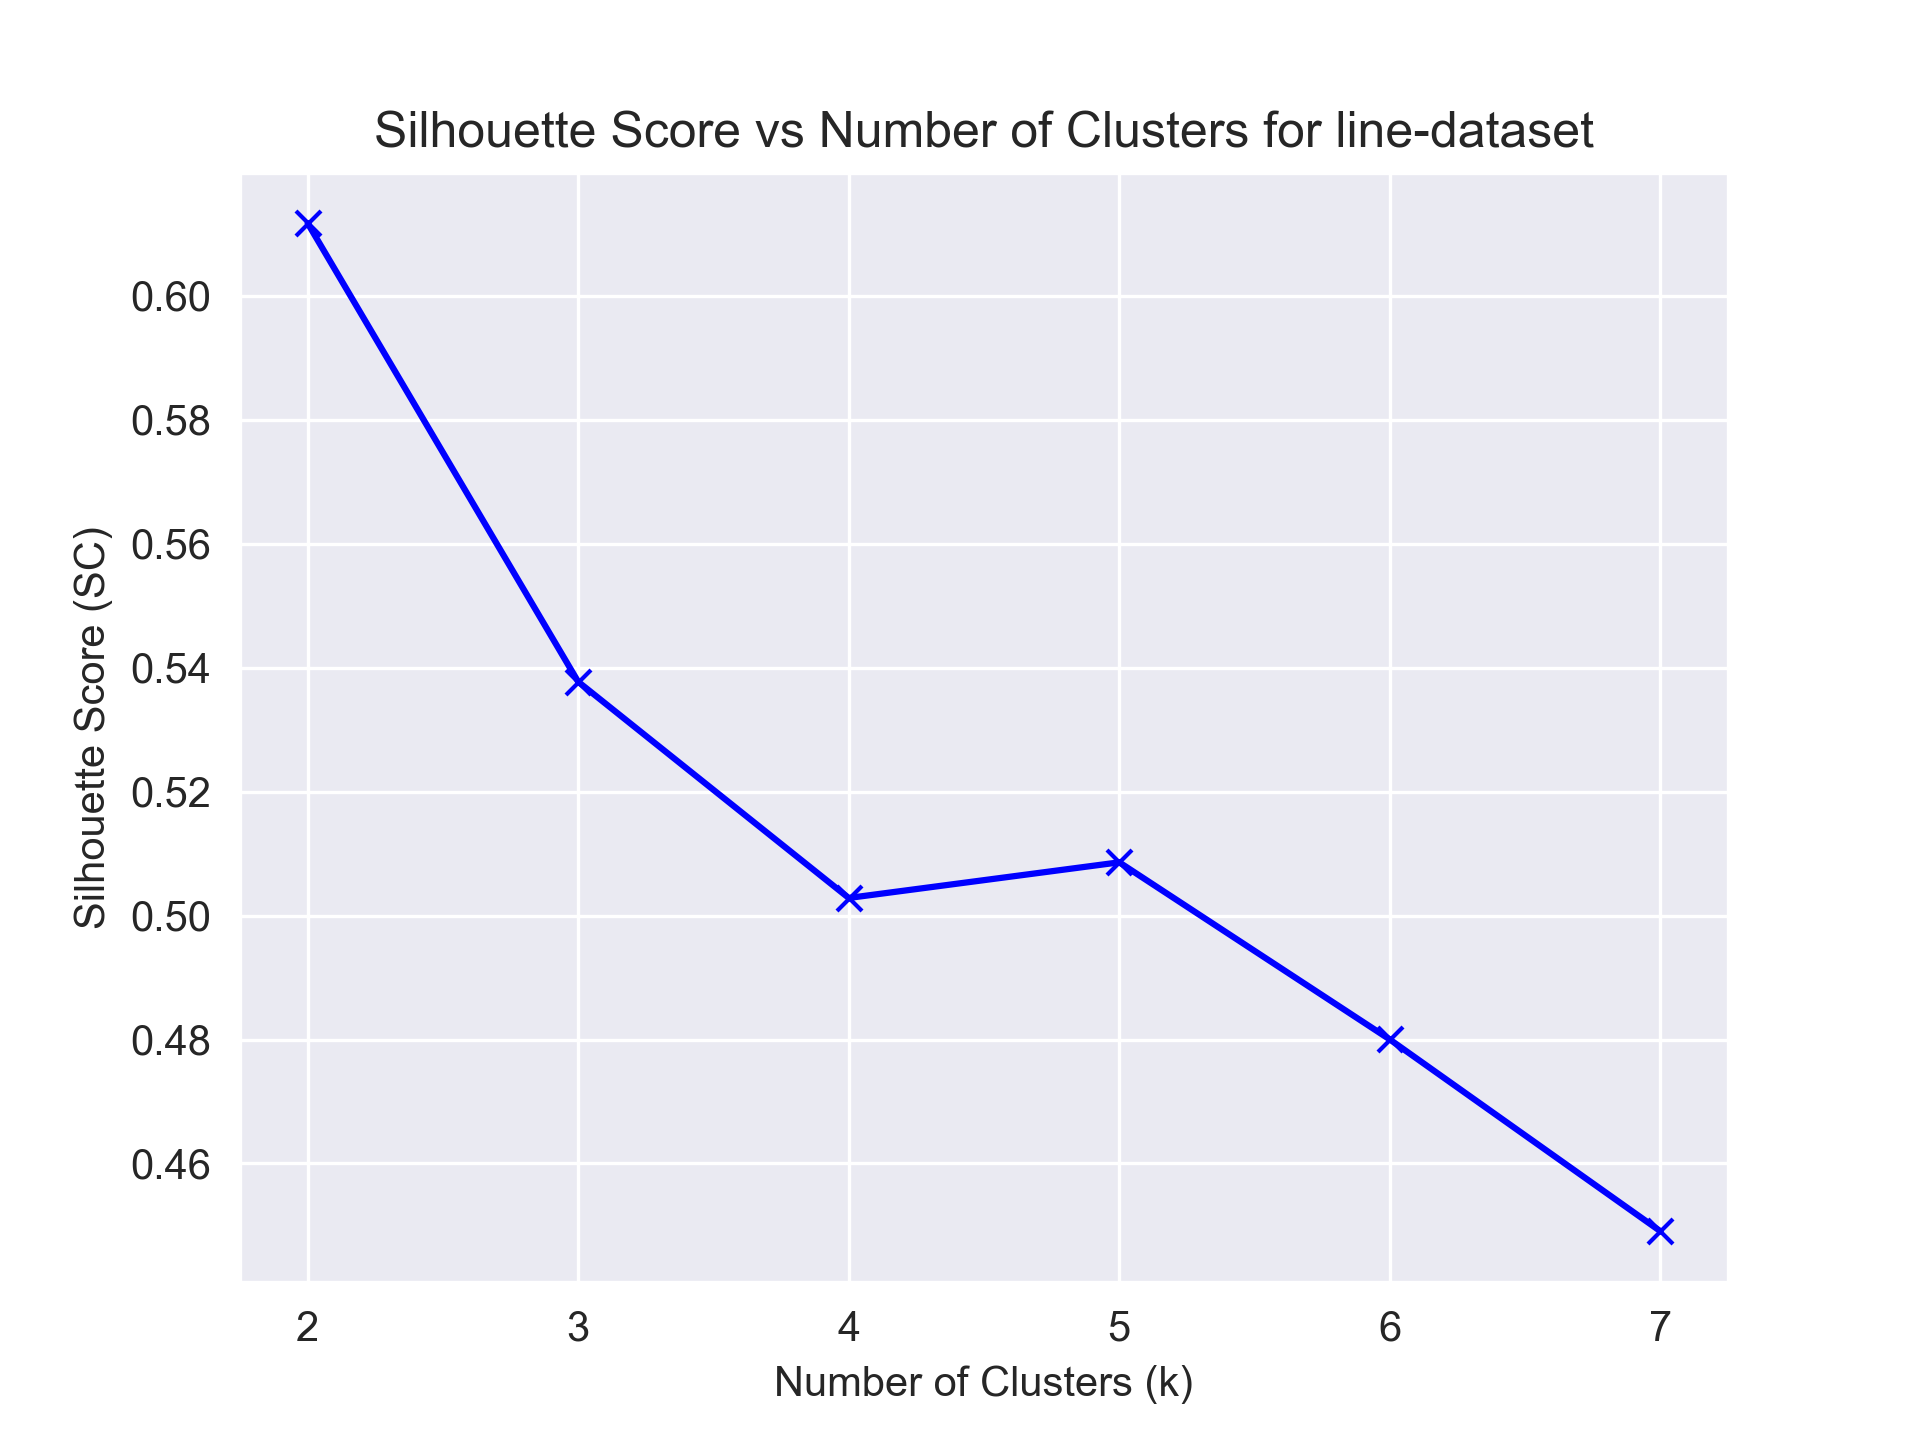
\includegraphics[width=0.8\textwidth]{Appendix/parameter-selection/line-dataset_agglomerative_optimal_cluster_2.png}
  \caption{Selecting the $k$ for Agglomerative clustering for line dataset (2-dimensions) using the "elbow plot."}
  \label{hyperparameters:agglomerative-line-dataset-2d}
\end{figure}
\begin{figure}[H]
  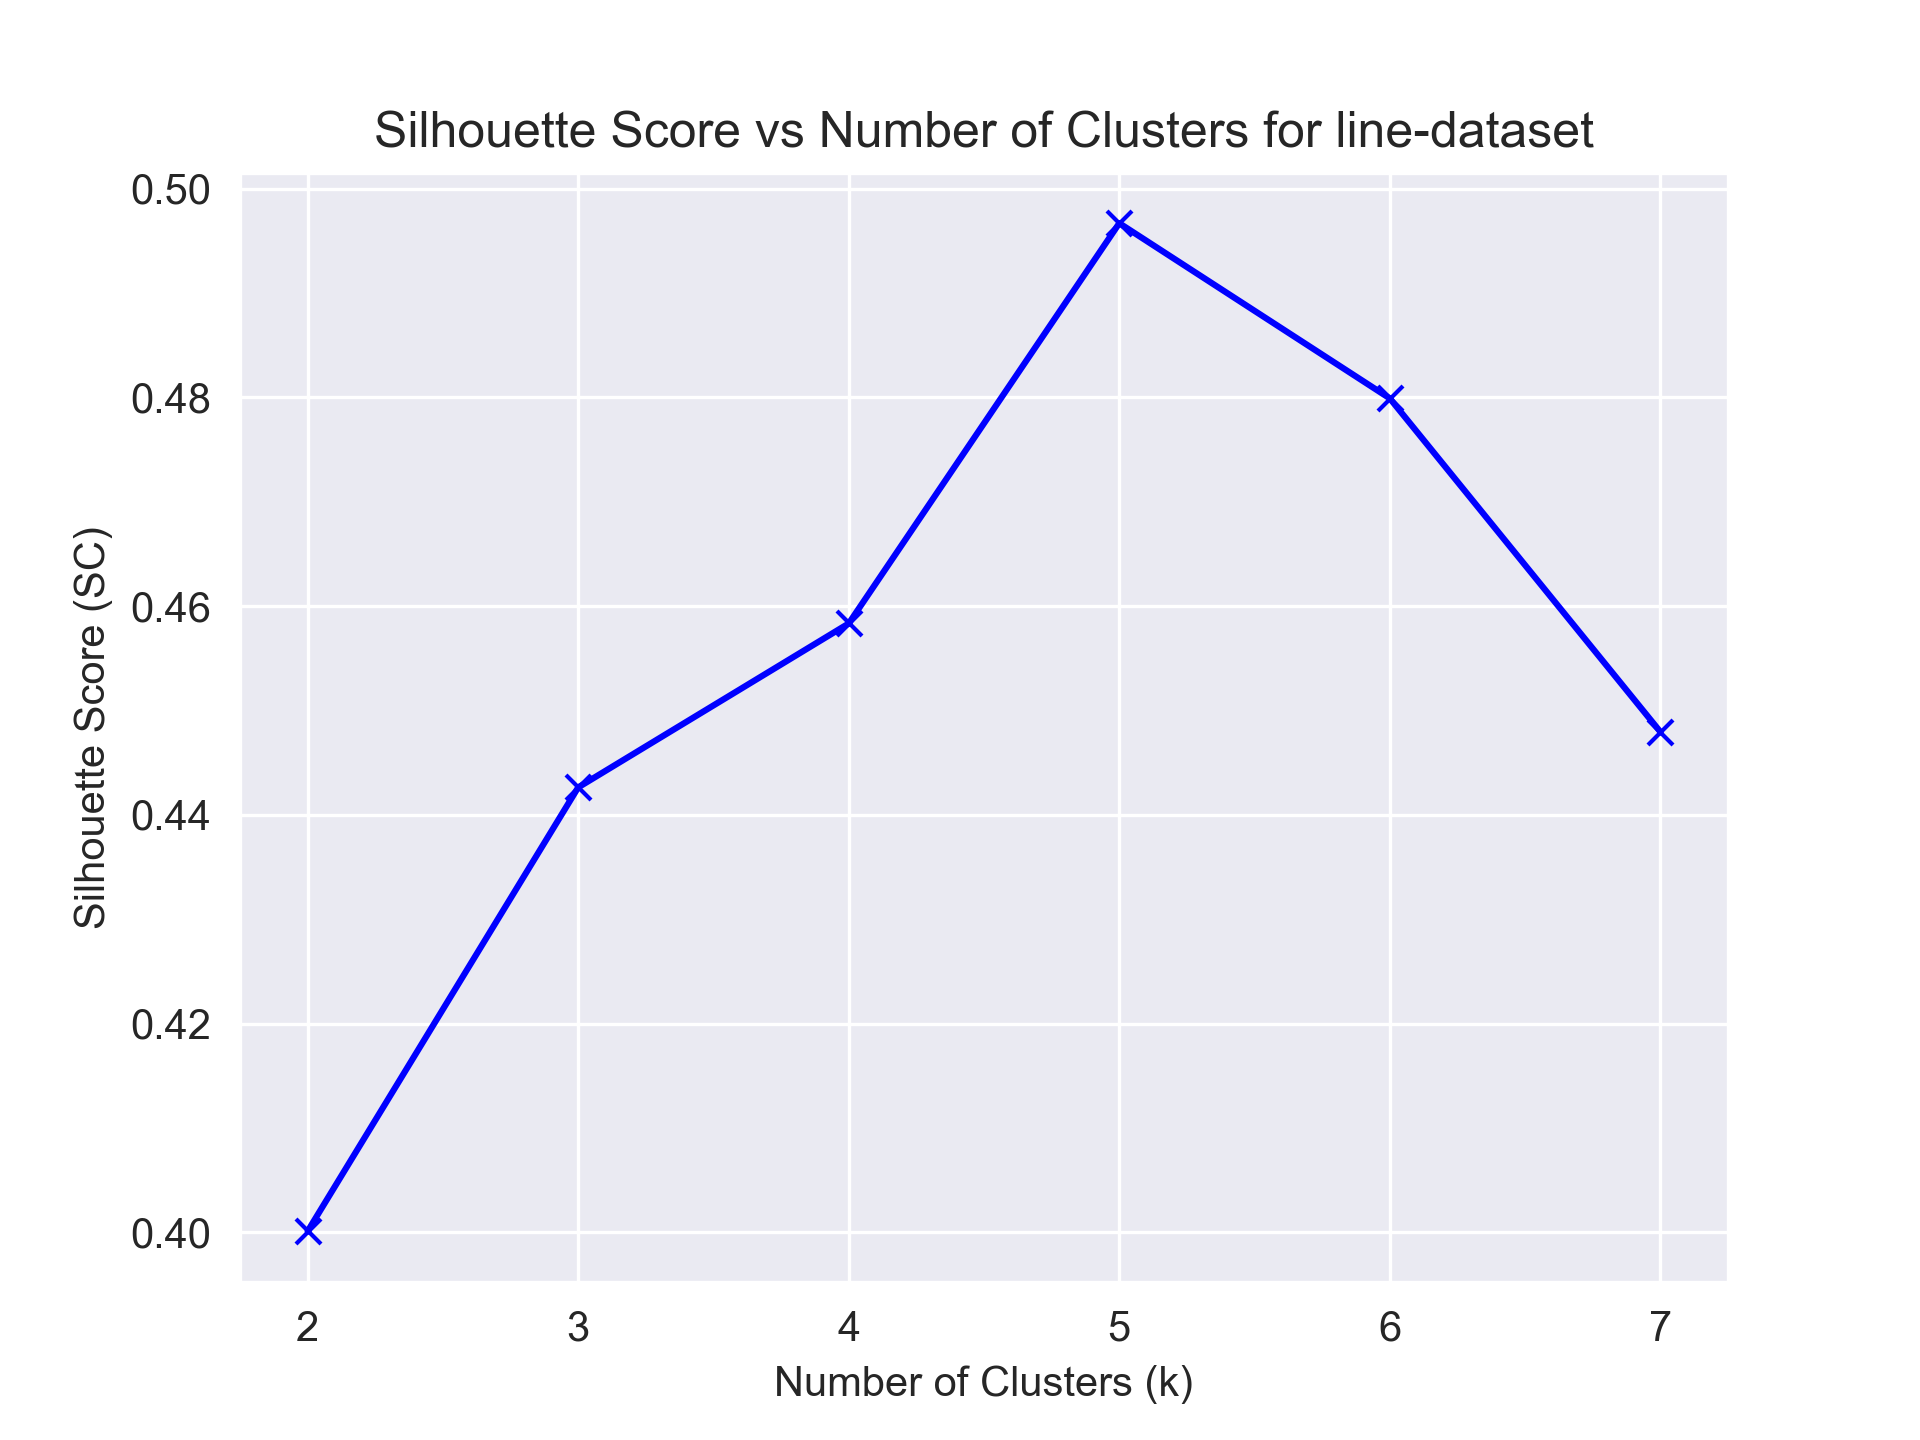
\includegraphics[width=0.8\textwidth]{Appendix/parameter-selection/line-dataset_agglomerative_optimal_cluster_3.png}
  \caption{Selecting the $k$ for Agglomerative clustering for line dataset (3-dimensions) using the "elbow plot."}
  \label{hyperparameters:agglomerative-line-dataset-3d}
\end{figure}
\newpage
\subsection{Skewed dataset}
\begin{figure}[H]
  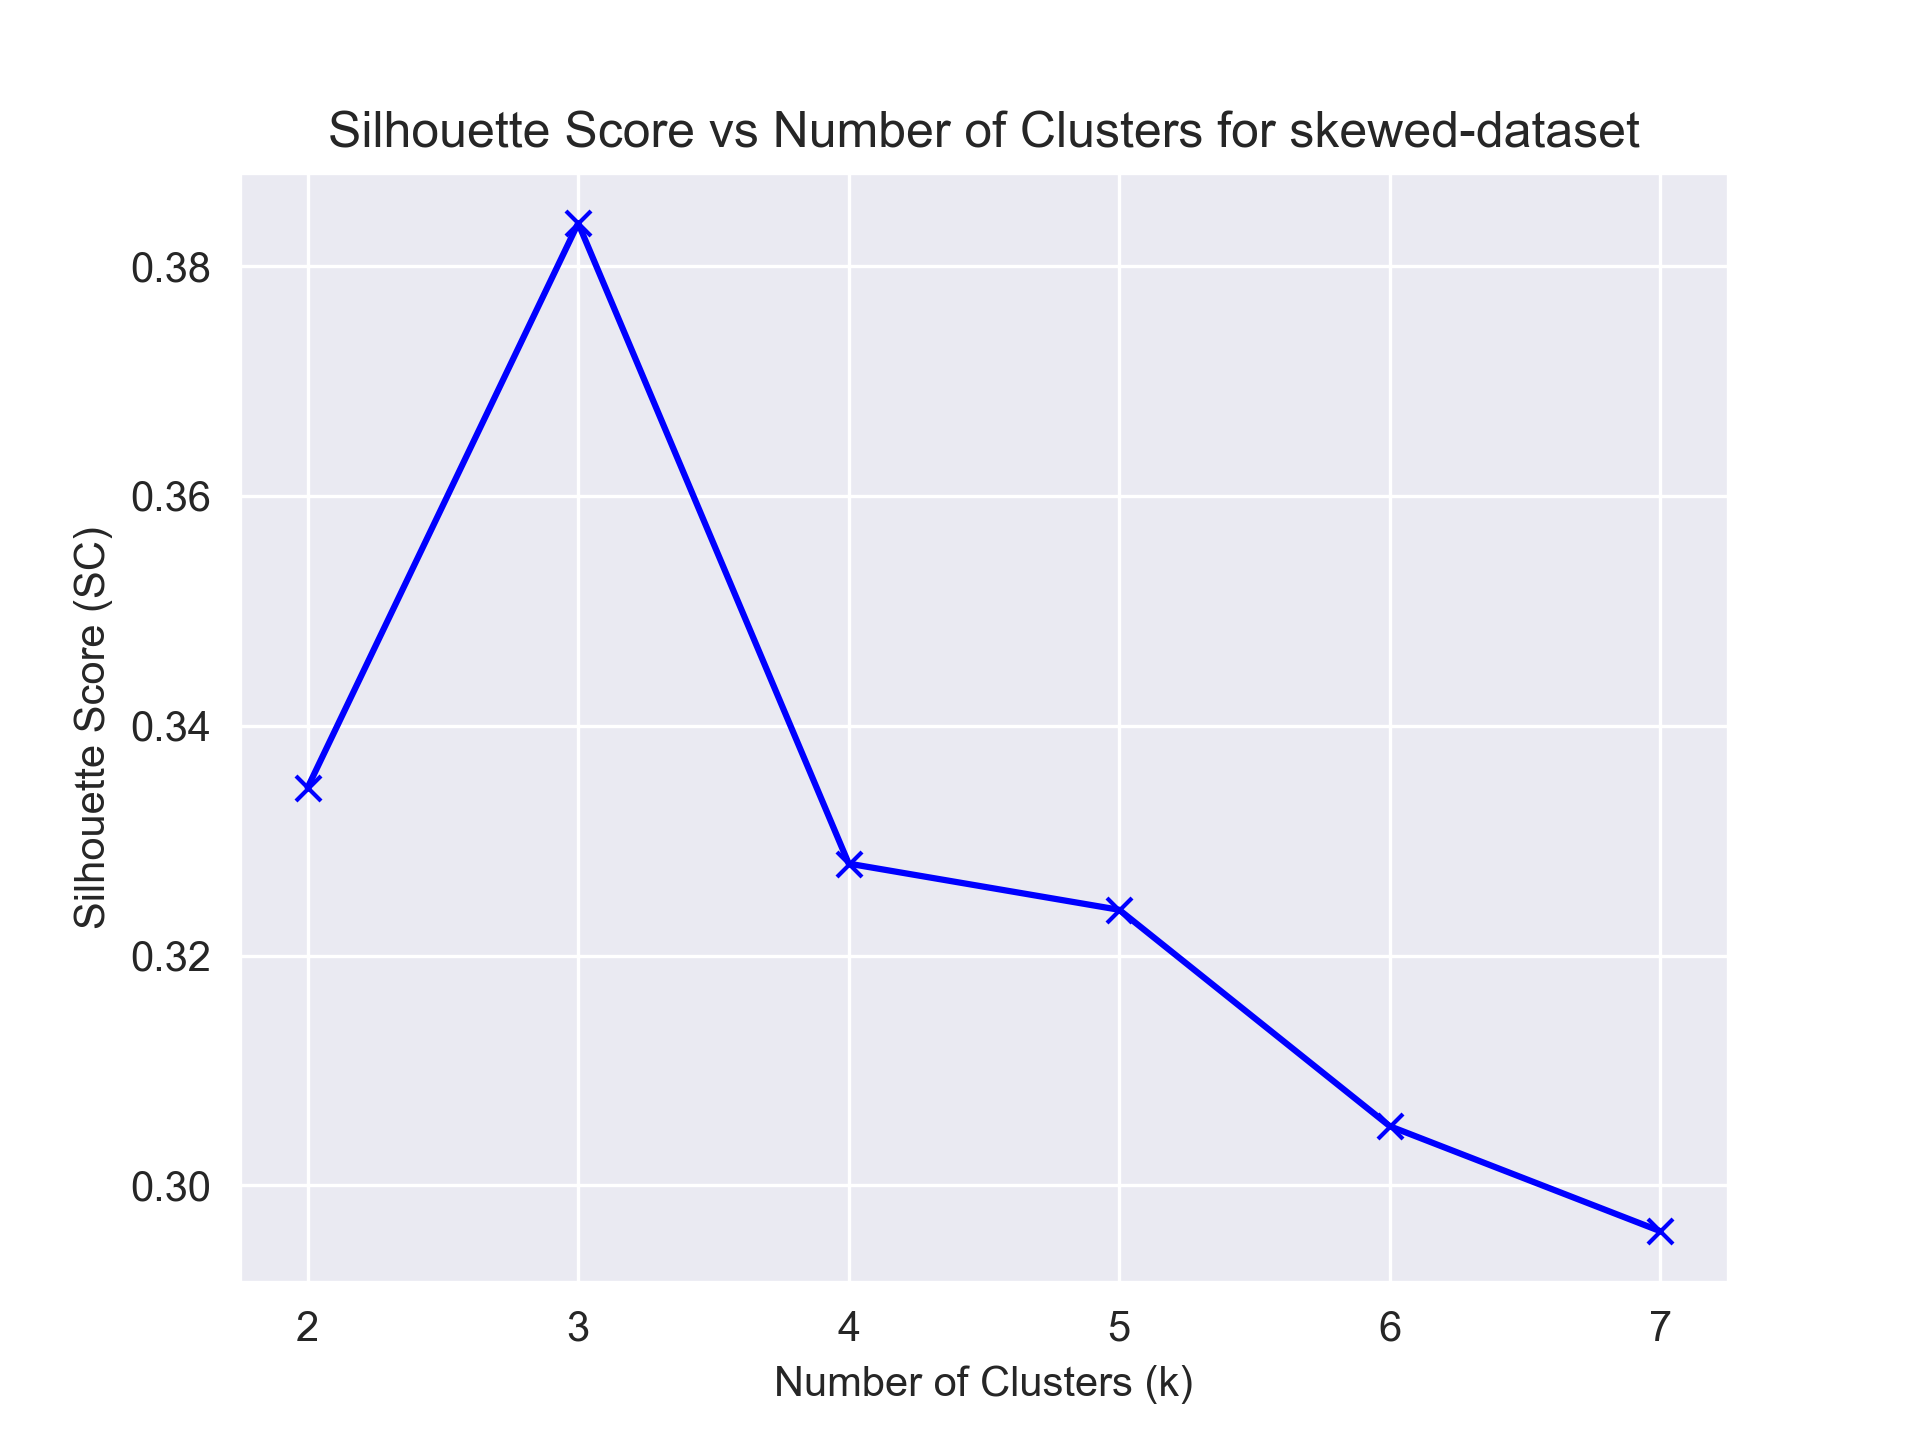
\includegraphics[width=0.8\textwidth]{Appendix/parameter-selection/skewed-dataset_agglomerative_optimal_cluster_2.png}
  \caption{Selecting the $k$ for Agglomerative clustering for skewed dataset (2-dimensions) using the "elbow plot."}
  \label{hyperparameters:agglomerative-skewed-dataset-2d}
\end{figure}
\begin{figure}[H]
  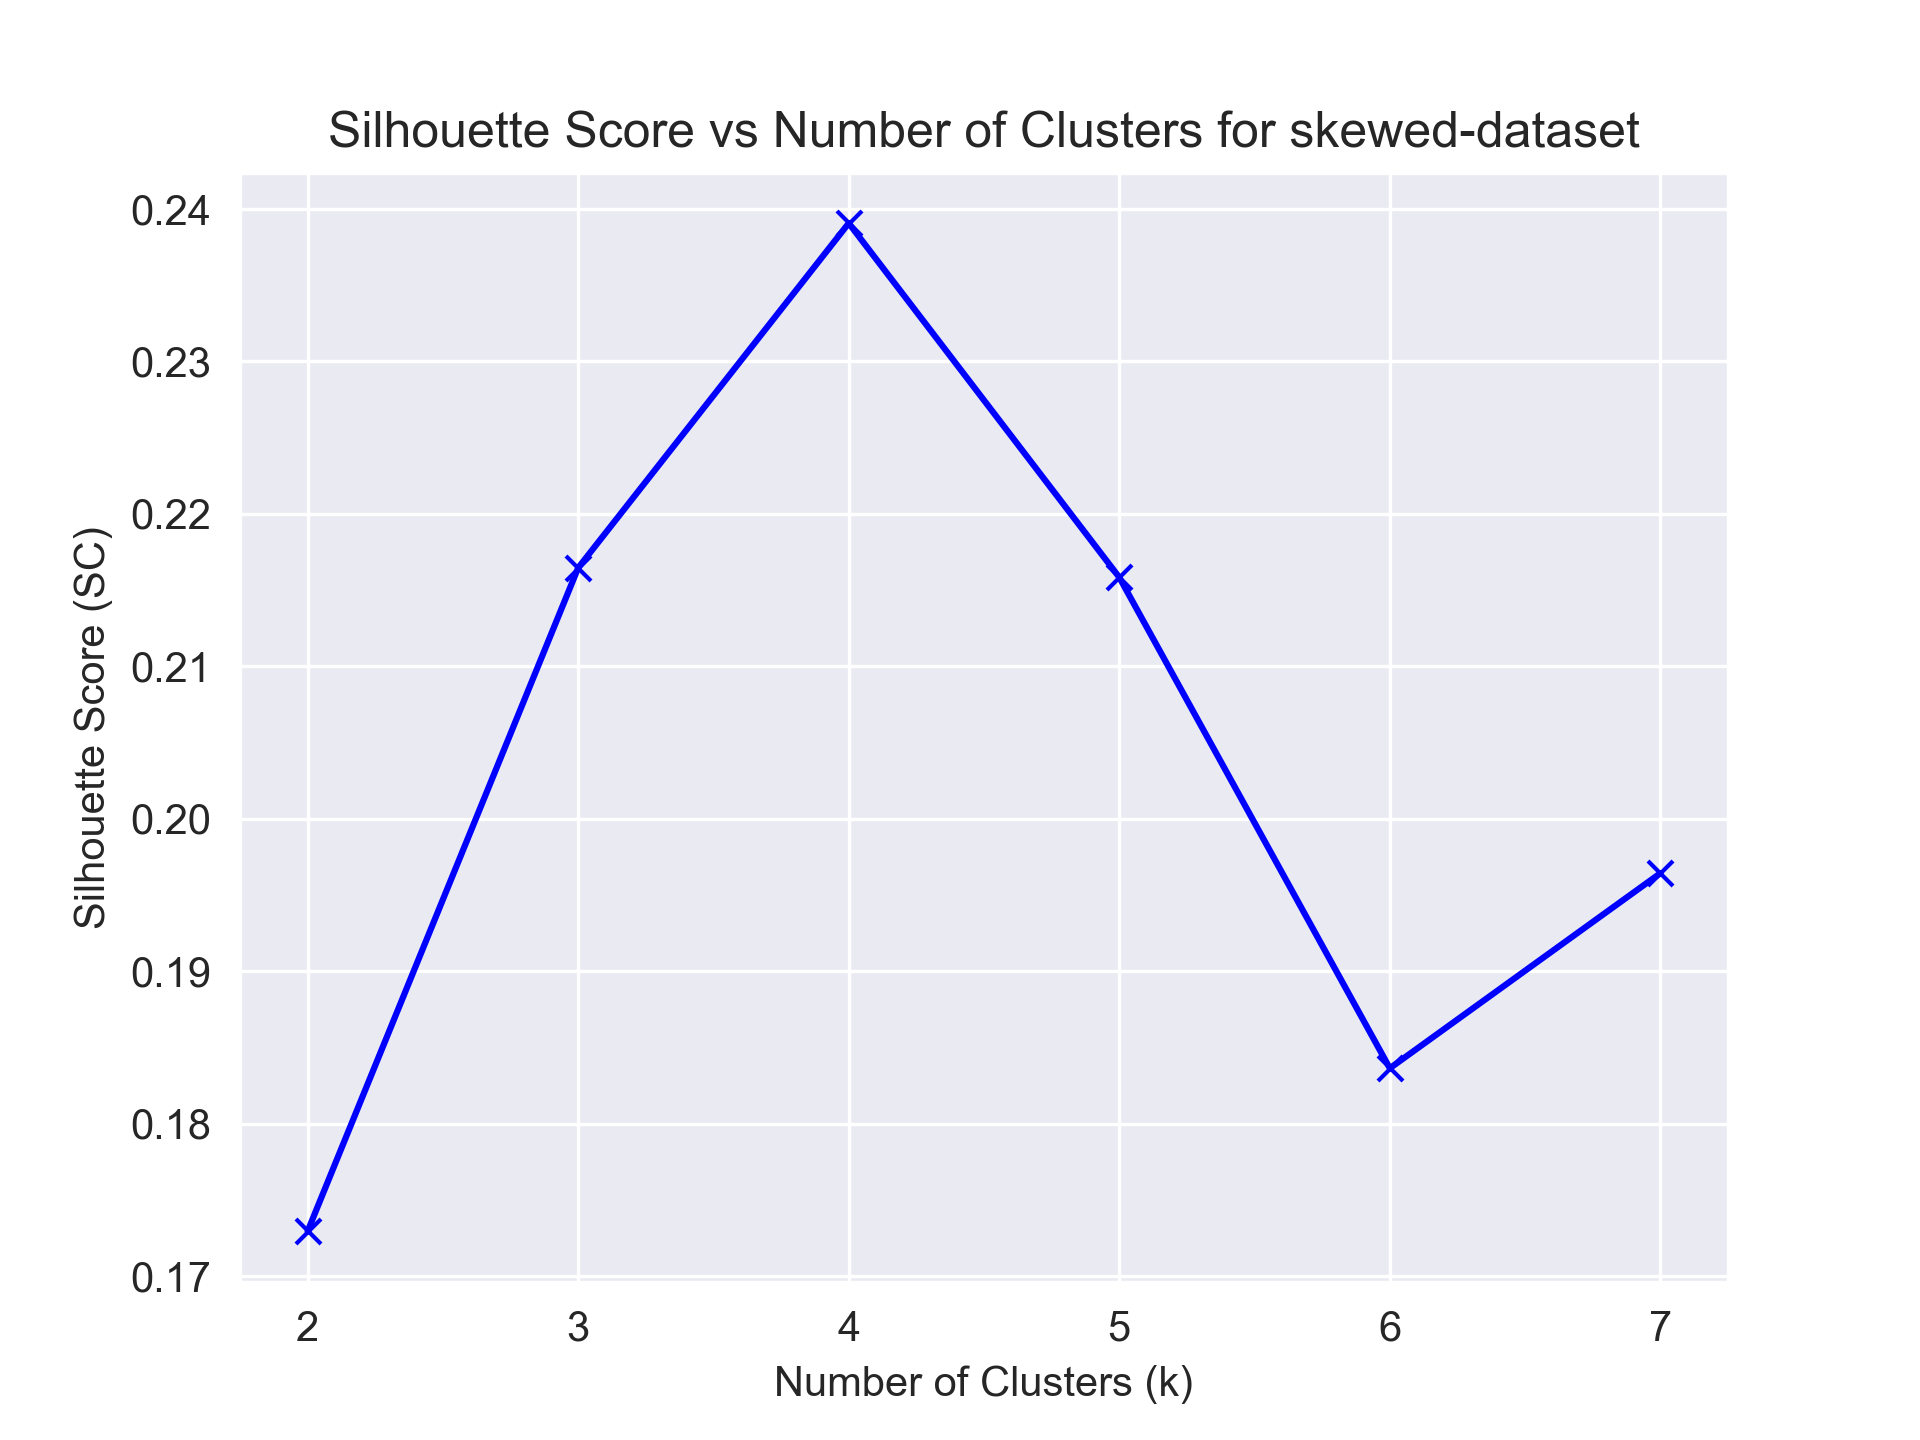
\includegraphics[width=0.8\textwidth]{Appendix/parameter-selection/skewed-dataset_agglomerative_optimal_cluster_3.png}
  \caption{Selecting the $k$ for Agglomerative clustering for skewed dataset (3-dimensions) using the "elbow plot."}
  \label{hyperparameters:agglomerative-skewed-dataset-3d}
\end{figure}